\documentclass[11pt]{ctexart}

\usepackage[a4paper,margin=2.8cm]{geometry}
\usepackage{amsmath}
\usepackage{amssymb}
\usepackage{graphicx}
\usepackage{booktabs}
\usepackage{longtable}
\usepackage{float}
\usepackage{xcolor}
\usepackage{listings}
\usepackage[colorlinks=true,linkcolor=blue,urlcolor=magenta,citecolor=blue]{hyperref}

\graphicspath{{../}}

\renewcommand{\figurename}{Figure}
\renewcommand{\tablename}{Table}

\definecolor{kwcolor}{rgb}{0,0.5,0}
\definecolor{strcolor}{rgb}{0.73,0.13,0.13}
\definecolor{cmtcolor}{rgb}{0.5,0.5,0.5}

\lstset{
  basicstyle=\ttfamily\footnotesize,
  numbers=left,
  numberstyle=\tiny\color{gray},
  keywordstyle=\color{kwcolor}\bfseries,
  commentstyle=\color{cmtcolor}\itshape,
  stringstyle=\color{strcolor},
  frame=lines,
  breaklines=true,
  postbreak=\mbox{\textcolor{gray}{$\hookrightarrow$}\space},
  showstringspaces=false,
  columns=fullflexible,
  xleftmargin=2.2em,
  framexleftmargin=1.6em,
  aboveskip=10pt,
  belowskip=10pt
}

\title{\textbf{图像频域水印实现报告}}
\author{题目 5 小组\quad 侯治民，乔义杰，金灏，王师睿\\[6pt]
\normalsize 代码仓库：\url{https://github.com/Mercury-LH/frequncy_domain_watermarking}}
\date{2026 年 5 月}

\begin{document}

\pagestyle{plain}

\maketitle

\section{引言}

\subsection{数字水印的背景}

随着数字图像在网络中的大规模传播，数字内容的版权保护、完整性验证和来源追踪变得日益重要。数字水印技术通过在原始媒体中嵌入标识信息，使该信息在正常观看时不可察觉，而在需要时可以通过算法提取出来，用于证明版权或追踪来源。一个实用的图像水印系统通常需要同时满足以下目标：

\begin{itemize}
  \item \textbf{不可见性}：水印嵌入后，含水印图像与原始图像在视觉上应尽量接近；
  \item \textbf{可提取性}：验证端能够从含水印图像中恢复出嵌入的水印信息；
  \item \textbf{鲁棒性}：图像经过 JPEG 压缩、缩放、噪声干扰等常见处理后，水印仍尽量可以恢复；
  \item \textbf{可扩展性}：算法应能处理不同尺寸、不同类型的图像，并能通过参数调节图像质量与水印强度之间的平衡。
\end{itemize}

与直接修改像素的空间域方法相比，频域水印先将图像变换到频域，再对频率系数施加受控扰动。由于压缩、滤波等图像处理操作本质上也是对频率成分的操作，频域水印更适合从信号与系统的角度分析不可见性与鲁棒性之间的关系，这也是本课程设置该题目的意义所在。

\subsection{频域水印的基本思想}

灰度图像可以视为二维离散信号 $f(x,y)$，$0 \le x < M$，$0 \le y < N$。频域水印的一般流程为：对图像施加某种可逆变换 $T$，在变换域中按规则修改一组系数，再通过逆变换 $T^{-1}$ 得到含水印图像，即
\begin{equation}
  I_w = T^{-1}\bigl(\, T(I) + \Delta \,\bigr),
  \label{eq:general}
\end{equation}
其中 $\Delta$ 是由水印比特决定的扰动。在频域中，低频系数对应图像的整体亮度与大尺度结构，修改低频容易产生可见失真；高频系数对应边缘与纹理细节，容易在压缩和滤波中被破坏。因此频域水印通常选择\textbf{中频区域}作为嵌入位置，在不可见性与鲁棒性之间取得折中。

\subsection{实验任务与目标}

本报告围绕图像频域水印的原理与实现，按照作业说明的基础、进阶、挑战三个层次完成了以下任务：

\begin{itemize}
  \item 实现 DFT 频域水印：对图像进行二维傅里叶变换，在频谱中频位置对称嵌入不可见水印，经逆变换得到含水印图像，并成功提取原始水印；
  \item 通过 MSE、PSNR、SSIM 指标验证水印不可见性，通过 NC、BER 指标衡量水印恢复质量；
  \item 分析嵌入强度对图像质量与提取准确率的影响，绘制强度--PSNR 与强度--BER 曲线；
  \item 测试水印在 JPEG 压缩、高斯噪声、缩放攻击下的鲁棒性，共 300 组攻击实验数据；
  \item 实现 DCT 域盲水印算法，提取水印不需要原始图像；
  \item 实现 DWT 小波域水印作为多分辨率变换域的扩展方案；
  \item 设计彩色图像 Y 通道水印接口，使彩色图像经水印处理后仍保持彩色；
  \item 构建模块化、可配置、带自动化测试的完整实验系统，全部实验可一键复现。
\end{itemize}

通过这些实验，我们不仅掌握了 DFT、DCT、DWT 三种变换的数学原理和代码实现，也直观体会到“修改一个频率系数，空间域会发生什么”这一课堂内容在真实工程问题中的表现。

\section{系统总体设计}

\subsection{项目结构与模块划分}

项目采用模块化结构组织代码，使算法实现、实验流程、指标计算和可视化输出相互独立。实验脚本不直接依赖具体算法类，而是通过注册表按名字创建算法对象；所有算法继承统一的抽象基类 \texttt{Watermarker}，只需实现 \texttt{embed} 与 \texttt{extract} 两个方法即可接入全部实验流程。整体目录如下：

\begin{lstlisting}
frequncy_domain_watermarking/
|-- configs/experiments.yaml      # 数据集、算法参数和实验参数
|-- data/
|   |-- images/                   # BSD 彩色图像
|   |-- misc/                     # USC-SIPI 灰度和彩色图像
|   `-- watermark/logo.png        # HJQ 水印图
|-- experiments/
|   |-- run_basic.py              # 基础实验
|   |-- run_strength.py           # 强度实验
|   |-- run_attacks.py            # 抗攻击实验
|   `-- run_all.py                # 一键运行全部实验
|-- src/watermarking/
|   |-- algorithms/               # base.py / dft.py / dct.py / dwt.py
|   |-- attacks.py                # JPEG、缩放、噪声攻击
|   |-- io_utils.py               # 图像读写、Y 通道处理
|   |-- metrics.py                # 图像质量与水印质量指标
|   |-- registry.py               # 算法注册表
|   `-- visualization.py          # 图像与曲线可视化
|-- tests/                        # 26 个 pytest 自动化测试
|-- main.py                       # 命令行接口 embed / extract / attack
`-- requirements.txt
\end{lstlisting}

所有实验参数集中在 \texttt{configs/experiments.yaml} 中，增删测试图、调整嵌入强度或攻击档位均不需要修改代码：

\begin{lstlisting}
methods:
  dft:  { alpha: 10.0, watermark_size: [64, 64], radius_ratio: 0.28 }
  dct:  { delta: 12.0, block_size: 8, watermark_size: [32, 32],
          coeff_pair: [[3, 4], [4, 3]] }
  dwt:  { alpha: 0.05, wavelet: haar, subband: hl, watermark_size: [64, 64] }
experiments:
  strengths: { dft: [2, 5, 10, 20, 40], dct: [2, 5, 10, 20, 40],
               dwt: [0.01, 0.03, 0.05, 0.1] }
  jpeg_qualities: [90, 70, 50, 30]
  noise_sigmas: [5, 10, 20]
  scale_factors: [0.5, 0.75, 1.5]
\end{lstlisting}

\subsection{数据集与水印}

实验使用 10 张测试图像，涵盖两种尺寸与两种存储格式，如 Table~\ref{tab:dataset} 所示。USC-SIPI 图像库提供 4 张 $512\times512$ 灰度图和 2 张 $512\times512$ 彩色图（无压缩 TIFF）；BSD 分割数据集提供 4 张 $481\times321$ 彩色图（有损 JPEG）。两类数据混合使用，在后续实验中暴露出了单一数据集难以观察到的现象（见 3.4 节）。

\begin{table}[H]
  \centering
  \caption{实验数据集}
  \label{tab:dataset}
  \begin{tabular}{llll}
    \toprule
    类型 & 数量 & 尺寸 & 图像名称 \\
    \midrule
    灰度图 & 4 & $512\times512$ & boat\_gray, gray21\_gray, texture\_gray, pattern\_gray \\
    彩色图 & 2 & $512\times512$ & house\_color, airplane\_color \\
    彩色图 & 4 & $481\times321$ & bsd\_color, bsd\_landscape\_color, bsd\_train\_color, bsd\_texture\_color \\
    \bottomrule
  \end{tabular}
\end{table}

水印为自制二值图像，内容为组员姓名首字母“HJQ”。嵌入前按各算法容量缩放并二值化：DFT 与 DWT 使用 $64\times64$，DCT 使用 $32\times32$。DCT 取更小尺寸是容量约束的结果：该方案每个 $8\times8$ 块承载 1 比特，$481\times321$ 的 BSD 图仅有 $60\times40=2400$ 个块，无法容纳 $64\times64=4096$ 比特，取 $32\times32=1024$ 比特后所有测试图均可容纳。

\subsection{评价指标}

不可见性通过三个图像质量指标衡量。均方误差 MSE 定义为
\begin{equation}
  \mathrm{MSE} = \frac{1}{MN}\sum_{x=0}^{M-1}\sum_{y=0}^{N-1}\bigl[I(x,y)-I_w(x,y)\bigr]^2,
  \label{eq:mse}
\end{equation}
峰值信噪比 PSNR 将其换算到对数尺度：
\begin{equation}
  \mathrm{PSNR} = 10\log_{10}\frac{255^2}{\mathrm{MSE}}\ (\mathrm{dB}),
  \label{eq:psnr}
\end{equation}
一般认为 PSNR 大于 40 dB 时失真难以察觉，30--40 dB 图像质量较好。结构相似性 SSIM 从亮度、对比度、结构三方面衡量两幅图像的相似程度：
\begin{equation}
  \mathrm{SSIM}(x,y) = \frac{(2\mu_x\mu_y + C_1)(2\sigma_{xy} + C_2)}{(\mu_x^2+\mu_y^2+C_1)(\sigma_x^2+\sigma_y^2+C_2)},
  \label{eq:ssim}
\end{equation}
取值越接近 1 表示结构越相似。

水印恢复质量通过两个指标衡量。归一化相关系数 NC 将原始水印 $W$ 与提取水印 $W'$ 映射为 $\pm1$ 序列后计算相关：
\begin{equation}
  \mathrm{NC} = \frac{\langle W, W'\rangle}{\lVert W\rVert\cdot\lVert W'\rVert},
  \label{eq:nc}
\end{equation}
比特错误率 BER 为提取比特与原始比特不一致的比例：
\begin{equation}
  \mathrm{BER} = \frac{\#\{\,i : w_i \ne w'_i\,\}}{n_{\mathrm{bits}}},
  \label{eq:ber}
\end{equation}
BER 为 0 表示完全正确，0.5 相当于随机猜测。

\subsection{运行环境}

实验在 macOS（Apple Silicon）环境下完成，Python 3.9.6。主要依赖为 numpy（FFT 与矩阵运算）、opencv-python（图像读写、DCT、颜色空间转换）、PyWavelets（DWT）、scikit-image（SSIM）、matplotlib、PyYAML 与 pandas，完整版本锁定于 \texttt{requirements.txt}。

\begin{lstlisting}[language=bash]
python3 -m pip install -r requirements.txt        # 安装依赖
python3 -m pytest -v                              # 运行 26 个自动化测试
PYTHONPATH=.:src python3 experiments/run_all.py   # 一键运行全部实验
\end{lstlisting}

\section{基础任务：DFT 频域水印}

\subsection{任务问题}

基础任务要求对图像进行 DFT 或类似频域变换，在频域特定位置嵌入不可见数字水印，通过逆变换得到含水印图像，再从中提取出原始水印，并验证不可见性。本节选择二维 DFT 作为基础算法。

\subsection{原理分析}

二维图像 $f(x,y)$ 的离散傅里叶变换及其逆变换为
\begin{equation}
  F(u,v) = \sum_{x=0}^{M-1}\sum_{y=0}^{N-1} f(x,y)\, e^{-j2\pi\left(\frac{ux}{M}+\frac{vy}{N}\right)},
  \label{eq:dft}
\end{equation}
\begin{equation}
  f(x,y) = \frac{1}{MN}\sum_{u=0}^{M-1}\sum_{v=0}^{N-1} F(u,v)\, e^{j2\pi\left(\frac{ux}{M}+\frac{vy}{N}\right)}.
  \label{eq:idft}
\end{equation}
实现中使用 \texttt{np.fft.fft2} 与 \texttt{np.fft.ifft2}，并用 \texttt{fftshift} 将零频移至频谱中心，以便按“到中心的距离”选择中频嵌入区域。

实值信号的频谱具有共轭对称性：
\begin{equation}
  F(u,v) = F^*\bigl((M-u)\bmod M,\ (N-v)\bmod N\bigr).
  \label{eq:conj}
\end{equation}
这一性质直接决定了嵌入方式：若只修改单个频点，逆变换结果将带有不可忽略的虚部，图像不再为实值。因此每写入一个扰动，必须同时在中心对称位置写入相同扰动，两个频点配对修改，逆变换的虚部才能相互抵消。

嵌入时先将水印比特映射为符号 $s\in\{-1,+1\}$（bit 1 对应 $+1$，bit 0 对应 $-1$），再对选定的中频位置施加
\begin{equation}
  F'(u,v) = F(u,v) + \beta\, s, \qquad \beta = \frac{\alpha M N}{32},
  \label{eq:embed}
\end{equation}
其中 $\alpha$ 为强度参数。提取时利用原图，对差值图像做 DFT：
\begin{equation}
  D(u,v) = \mathcal{F}\{I_w - I\},
  \label{eq:extract}
\end{equation}
理想情况下 $D$ 在嵌入位置只剩 $\pm\beta$，取其实部符号即可恢复比特。该方案提取需要原图，属于非盲水印。

\subsection{算法设计与实现}

嵌入流程为：读取图像并转为灰度矩阵 $\rightarrow$ 水印缩放二值化 $\rightarrow$ 二维 FFT 并中心化 $\rightarrow$ 在 \texttt{radius\_ratio} 决定的中频环带内选取 4096 个嵌入位置（跳过与自身镜像重合的点）$\rightarrow$ 按式~\eqref{eq:embed} 成对写入扰动 $\rightarrow$ 逆 FFT 取实部得到含水印图像。核心代码如下：

\begin{lstlisting}[language=Python]
def embed(self, image, watermark):
    host = ensure_grayscale_float(image)
    bits = watermark_to_bits(watermark)
    signs = bits.astype(np.float64) * 2 - 1
    spectrum = np.fft.fftshift(np.fft.fft2(host))
    positions = self._positions(host.shape, bits.shape)
    height, width = host.shape
    strength = self.alpha * height * width / 32.0
    for idx, (y, x) in enumerate(positions):
        spectrum[y, x] += strength * signs.ravel()[idx]
        spectrum[(height - y) % height, (width - x) % width] \
            += strength * signs.ravel()[idx]
    watermarked = np.fft.ifft2(np.fft.ifftshift(spectrum)).real
    return WatermarkResult(image=normalize_uint8(watermarked), ...)
\end{lstlisting}

式~\eqref{eq:embed} 中扰动幅度 $\beta$ 与图像尺寸 $MN$ 挂钩是实现中的一个关键设计。早期版本直接使用固定幅度 $\alpha$，提取结果接近随机噪声：由式~\eqref{eq:dft} 可知 DFT 系数是全图求和而非平均，$512\times512$ 图像的中频系数幅值可达数万量级，固定的小扰动完全淹没在浮点图像取整回 uint8 的舍入噪声中。将强度按 $MN$ 缩放后，同一 $\alpha$ 在不同尺寸图像上才具有可比的嵌入效果。

提取按式~\eqref{eq:extract} 实现，仅需数行：

\begin{lstlisting}[language=Python]
def extract(self, image, watermark_shape, original_image=None):
    if original_image is None:
        raise ValueError("DFT extraction requires original_image.")
    watermarked = ensure_grayscale_float(image)
    original = ensure_grayscale_float(original_image)
    difference = np.fft.fftshift(np.fft.fft2(watermarked - original))
    positions = self._positions(watermarked.shape, watermark_shape)
    bits = np.array([1 if difference[y, x].real >= 0 else 0
                     for y, x in positions], dtype=np.uint8)
    return ExtractionResult(
        watermark=(bits.reshape(watermark_shape) * 255).astype(np.uint8),
        metadata={"method": self.method_name, "blind": False})
\end{lstlisting}

\subsection{运行结果与分析}

Figure~\ref{fig:dft-boat} 给出 $512\times512$ 灰度图 boat 上的 DFT 结果，五联图依次为原图、含水印图、差异图、原始水印与提取水印；Figure~\ref{fig:dft-boat-spec} 为对应的频谱对比，可以直接观察到嵌入前后中频环带的变化。

\begin{figure}[H]
  \centering
  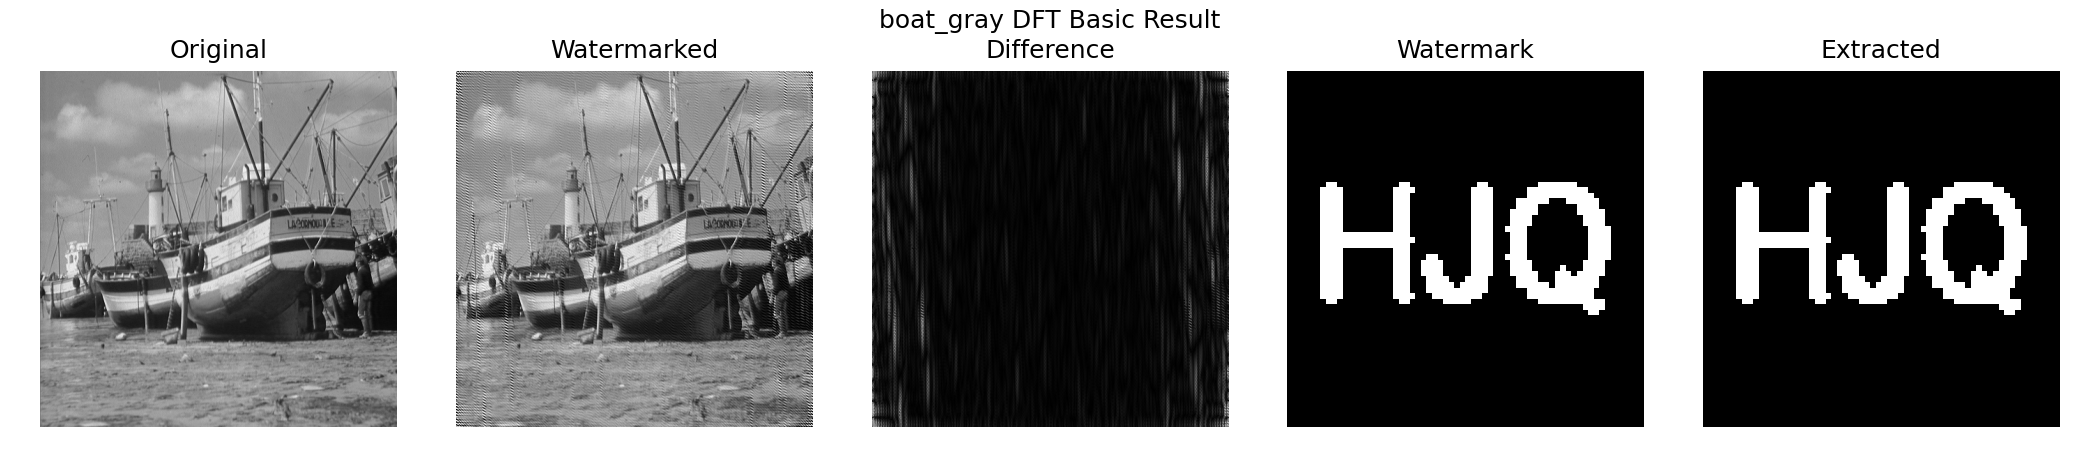
\includegraphics[width=0.95\textwidth]{outputs/multi_image/basic/boat_gray/dft_comparison.png}
  \caption{boat\_gray 的 DFT 嵌入与提取结果}
  \label{fig:dft-boat}
\end{figure}

\begin{figure}[H]
  \centering
  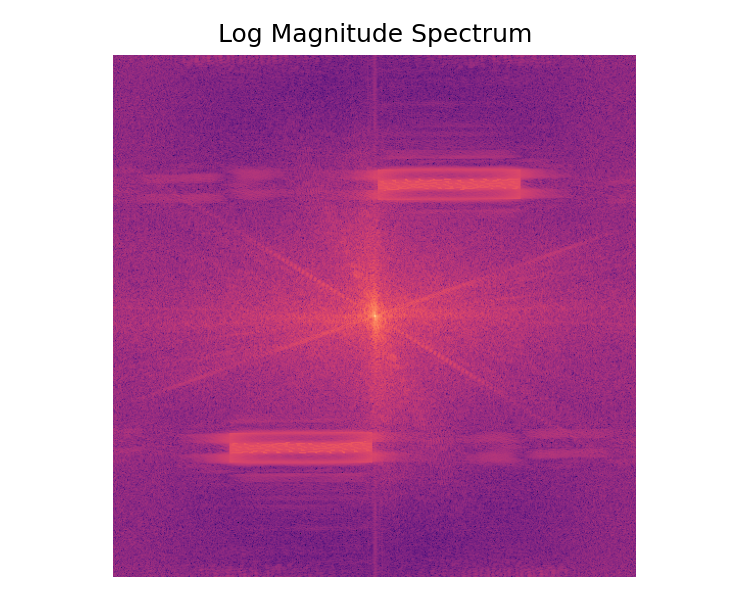
\includegraphics[width=0.8\textwidth]{outputs/multi_image/basic/boat_gray/dft_spectrum.png}
  \caption{boat\_gray 的 DFT 频谱对比（嵌入前后）}
  \label{fig:dft-boat-spec}
\end{figure}

\begin{figure}[H]
  \centering
  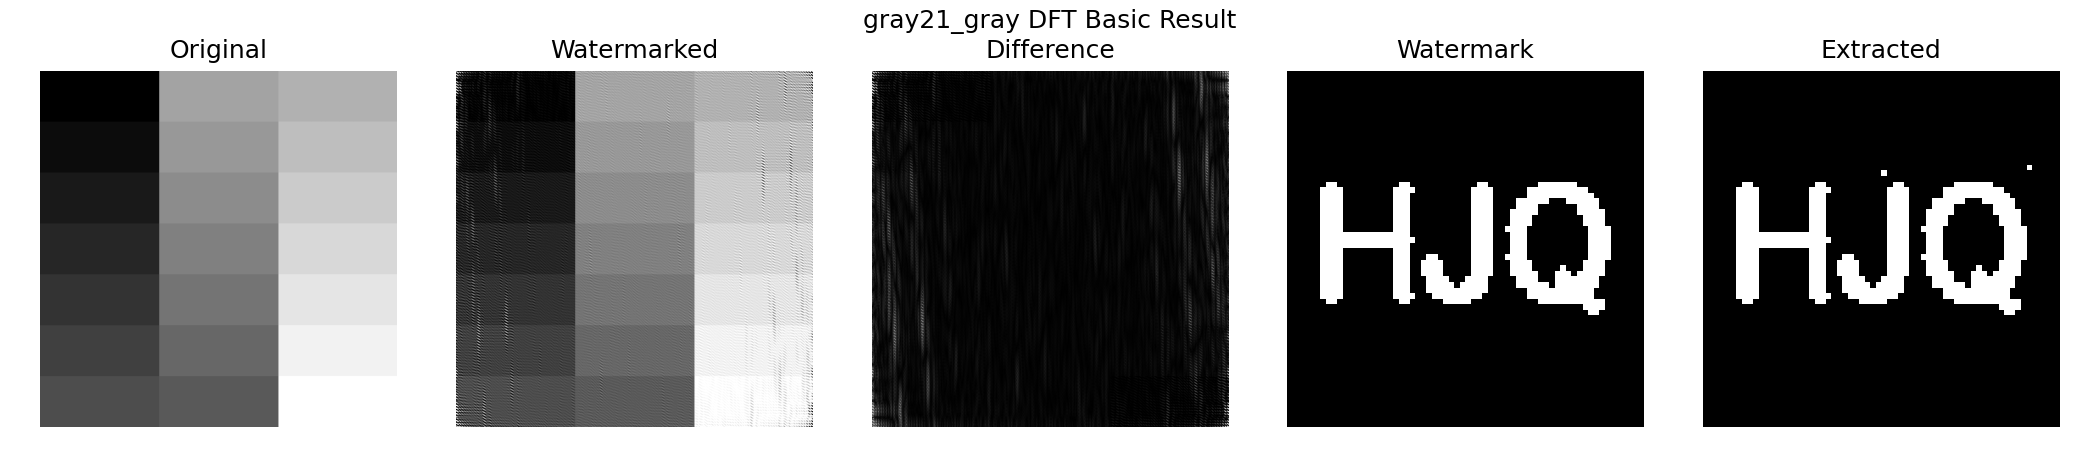
\includegraphics[width=0.95\textwidth]{outputs/multi_image/basic/gray21_gray/dft_comparison.png}
  \caption{gray21\_gray 的 DFT 结果}
  \label{fig:dft-gray21}
\end{figure}

\begin{figure}[H]
  \centering
  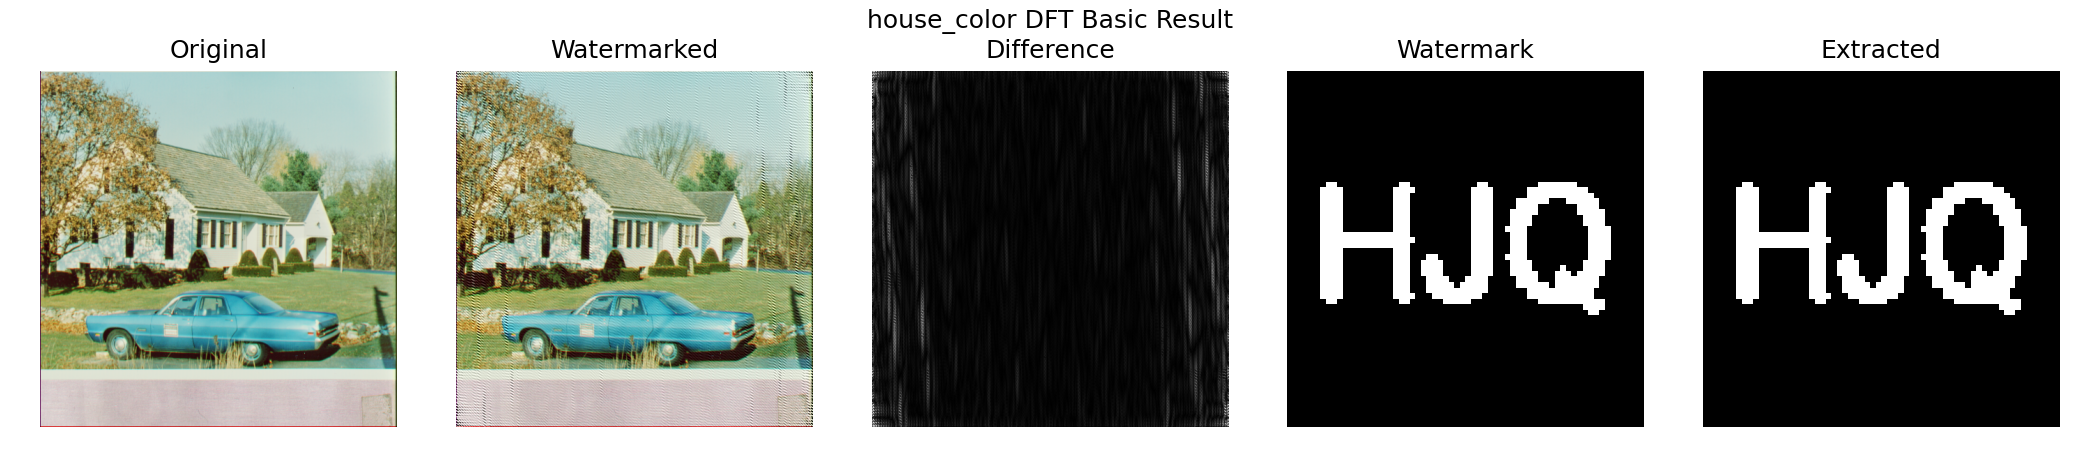
\includegraphics[width=0.95\textwidth]{outputs/multi_image/basic/house_color/dft_comparison.png}
  \caption{house\_color 的 DFT 结果（经 Y 通道处理，输出保持彩色）}
  \label{fig:dft-house}
\end{figure}

定量结果方面，四张 $512\times512$ 灰度图的提取全部无差错（BER = 0，NC = 1.0），boat 的 PSNR 为 22.95 dB，gray21 为 23.60 dB。该 PSNR 处于“有一定失真”区间：在 gray21 这类大面积平坦的图像上，差异图中可以观察到轻微的波纹状扰动。$\alpha=10$ 是权衡后的默认值——第 8 节的强度实验表明 $\alpha$ 降至 2 时 PSNR 可达 35 dB，但留给后续攻击实验的判决余量将明显减小。基础任务优先保证提取的稳定性，因此接受了这一失真水平。

一个值得注意的现象是：三张 $481\times321$ 的 BSD 图上 DFT 的 BER 升至 8.7\%--10.1\%，而同为彩色、尺寸为 $512\times512$ 的 house 与 airplane 仍为 0。差别不在彩色处理而在尺寸奇偶性：481 与 321 均为奇数，\texttt{fftshift} 后的频谱中心与共轭对称的真实中心相差半个像素，按 $(M-u)\bmod M$ 计算的镜像位置存在系统性错位，部分对称扰动未能精确配对，逆变换丢弃虚部时损失了嵌入信息。该解释与“偶数尺寸全对、奇数尺寸出错”的实验规律吻合，是本实现已定位但尚未修复的局限。

\section{挑战任务一：DCT 盲水印算法}

\subsection{任务问题}

挑战任务要求尝试 DCT 或 DWT 域水印，并设计\textbf{盲水印}算法——提取水印时不依赖原始图像。本节将 DCT 作为主要盲水印方案。DCT 广泛用于图像压缩（JPEG 标准的核心变换），图像划分为 $8\times8$ 块后，每块经 DCT 得到 64 个频率系数，左上角为低频，右下角为高频，中间区域为中频。

\subsection{原理分析}

$N\times N$ 图像块的二维 DCT 为
\begin{equation}
  C(u,v) = \alpha(u)\alpha(v)\sum_{x=0}^{N-1}\sum_{y=0}^{N-1} f(x,y)
  \cos\frac{(2x+1)u\pi}{2N}\cos\frac{(2y+1)v\pi}{2N}.
  \label{eq:dct}
\end{equation}

盲提取的约束决定了编码方式：提取端没有参照物，“嵌入时加了多少、提取时减回来”的思路不可行。解决办法是不记录系数的\textbf{绝对值}，而记录两个系数之间的\textbf{相对大小关系}。在每块中选取两个地位对称的中频系数 $c_1 = C(3,4)$、$c_2 = C(4,3)$，编码规则为
\begin{equation}
  \text{bit} = 1 \Leftrightarrow c_1 > c_2, \qquad
  \text{bit} = 0 \Leftrightarrow c_1 < c_2.
  \label{eq:dct-rule}
\end{equation}
提取时重新分块、重新做 DCT、比较同一对系数即可恢复比特，全程不需要原图。选取 $(3,4)$ 与 $(4,3)$ 的原因是二者位于 zigzag 扫描的同一反对角线上，频率高低相同，在 JPEG 标准量化表中对应的量化步长也几乎一致，先验上两系数的大小关系接近随机，交换顺序不会给图像带来方向性偏差。

\subsection{算法设计与实现}

嵌入时将两个系数移至其中点，再向两侧各推开 $\delta/2$，保证顺序正确且间距至少为 $\delta$：

\begin{lstlisting}[language=Python]
def embed(self, image, watermark):
    host = ensure_grayscale_float(image).copy()
    bits = watermark_to_bits(watermark).ravel()
    if bits.size > self._capacity(host.shape):
        raise ValueError("watermark exceeds DCT capacity")
    c1, c2 = self.coeff_pair
    for bit, (y, x, block) in zip(bits, self._iter_blocks(host)):
        dct_block = cv2.dct(block.astype(np.float32))
        midpoint = (dct_block[c1] + dct_block[c2]) / 2.0
        if bit == 1:
            dct_block[c1] = midpoint + self.delta / 2.0
            dct_block[c2] = midpoint - self.delta / 2.0
        else:
            dct_block[c1] = midpoint - self.delta / 2.0
            dct_block[c2] = midpoint + self.delta / 2.0
        host[y:y+8, x:x+8] = cv2.idct(dct_block)
    return WatermarkResult(image=normalize_uint8(host), ...)
\end{lstlisting}

参数 $\delta$ 即该算法的嵌入强度：间距越大，越能承受后续处理造成的系数漂移，代价是块内失真增大。提取只需比较系数：

\begin{lstlisting}[language=Python]
def extract(self, image, watermark_shape, original_image=None):
    host = ensure_grayscale_float(image)
    c1, c2 = self.coeff_pair
    bits = []
    for _, _, block in self._iter_blocks(host):
        dct_block = cv2.dct(block.astype(np.float32))
        bits.append(1 if dct_block[c1] > dct_block[c2] else 0)
        if len(bits) == int(np.prod(watermark_shape)):
            break
    return ExtractionResult(
        watermark=(np.array(bits, dtype=np.uint8)
                   .reshape(watermark_shape) * 255).astype(np.uint8),
        metadata={"method": self.method_name, "blind": True})
\end{lstlisting}

\subsection{运行结果与分析}

\begin{figure}[H]
  \centering
  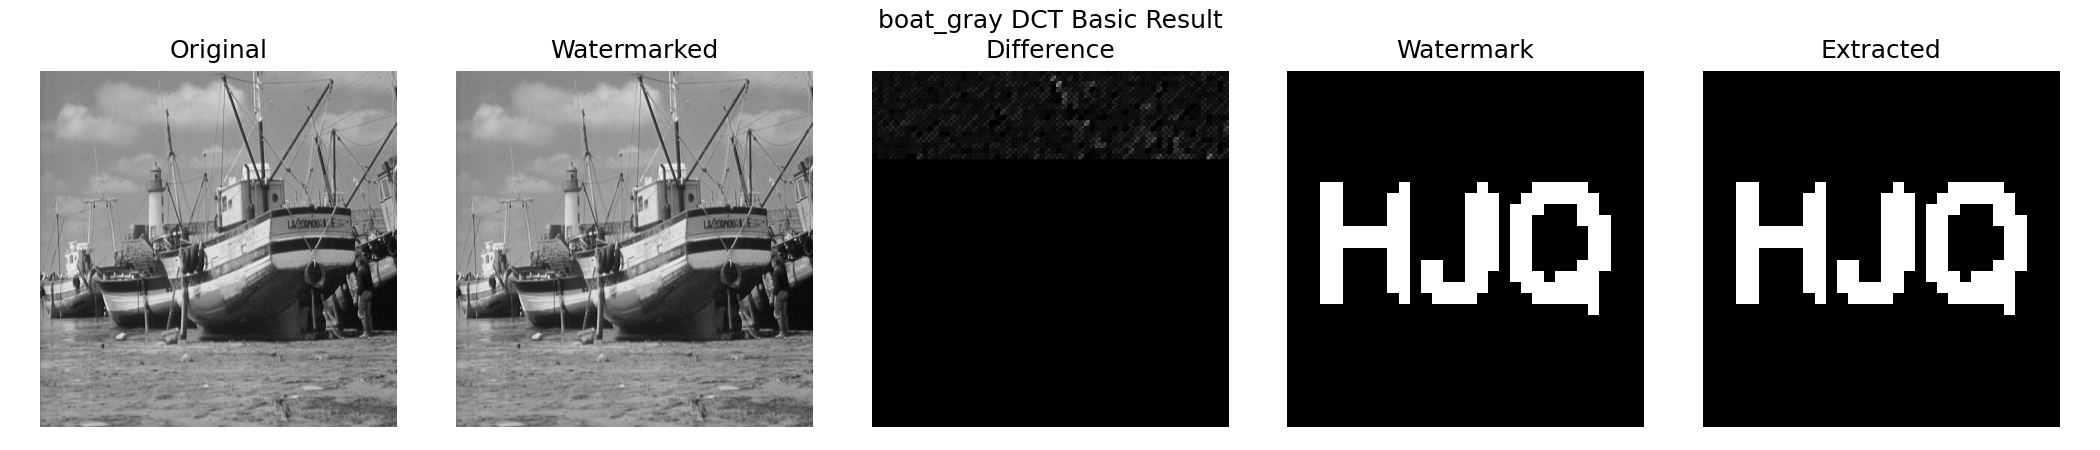
\includegraphics[width=0.95\textwidth]{outputs/multi_image/basic/boat_gray/dct_comparison.png}
  \caption{boat\_gray 的 DCT 盲水印结果}
  \label{fig:dct-boat}
\end{figure}

\begin{figure}[H]
  \centering
  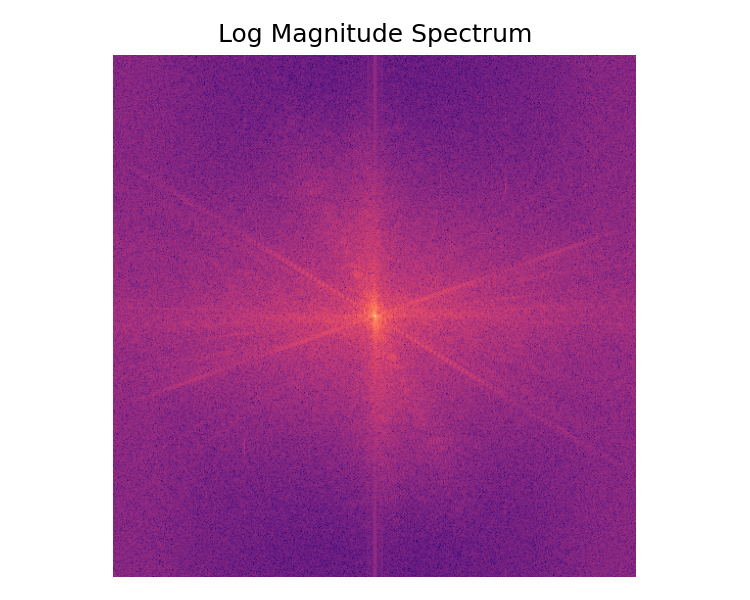
\includegraphics[width=0.8\textwidth]{outputs/multi_image/basic/boat_gray/dct_spectrum.png}
  \caption{boat\_gray 的 DCT 频谱可视化}
  \label{fig:dct-boat-spec}
\end{figure}

\begin{figure}[H]
  \centering
  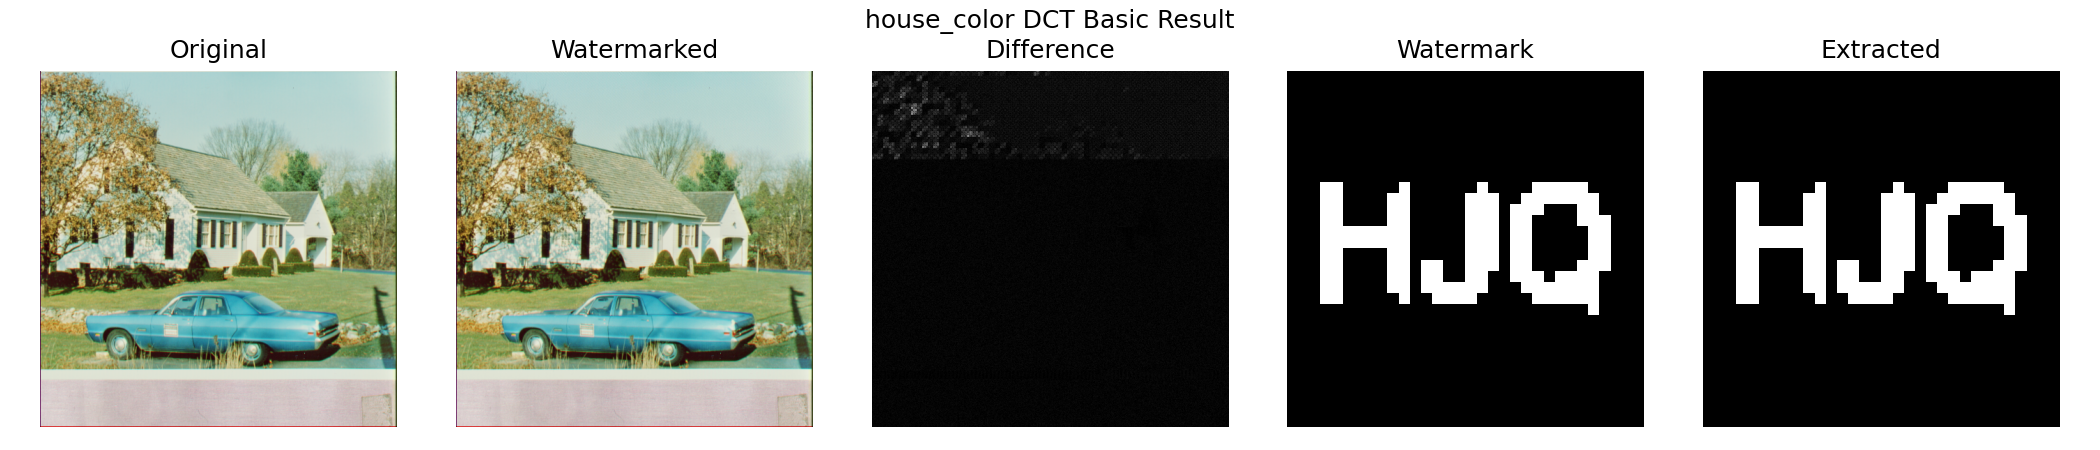
\includegraphics[width=0.95\textwidth]{outputs/multi_image/basic/house_color/dct_comparison.png}
  \caption{house\_color 的 DCT 盲水印结果}
  \label{fig:dct-house}
\end{figure}

\begin{figure}[H]
  \centering
  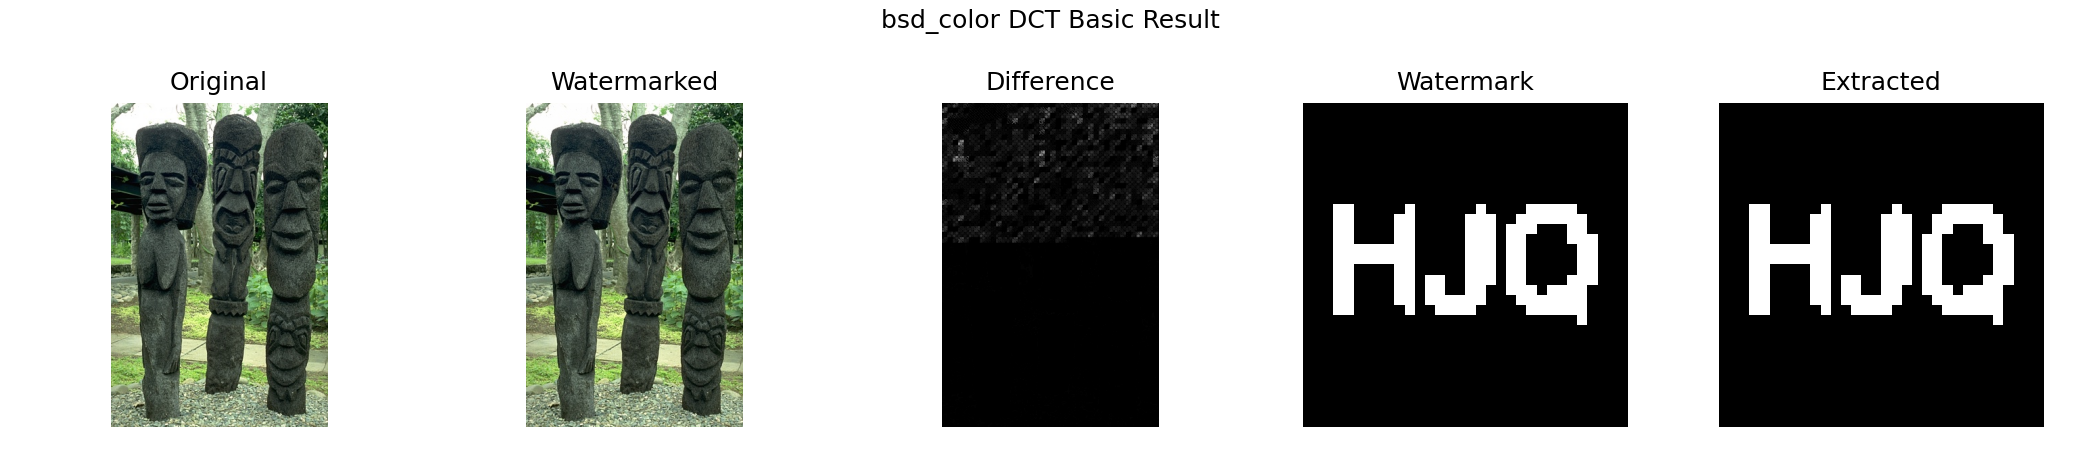
\includegraphics[width=0.95\textwidth]{outputs/multi_image/basic/bsd_color/dct_comparison.png}
  \caption{bsd\_color 的 DCT 盲水印结果}
  \label{fig:dct-bsd}
\end{figure}

不可见性方面 DCT 是三种方法中最好的：10 张图的平均 PSNR 达 47.54 dB（最低的 airplane 为 42.63 dB，最高的 gray21 为 53.96 dB），平均 SSIM 为 0.9957，差异图上几乎观察不到结构化痕迹。提取方面，10 张图中 9 张 BER 为 0。

唯一的例外是 pattern\_gray，BER 为 1.27\%。分析原因：该图含有大面积完全平坦的区域，这些块的中频系数原本全为 0，嵌入后 $c_1$、$c_2$ 仅为 $\pm\delta/2=\pm6$ 的小量，而 IDCT 回像素域并取整为 uint8 的过程中，如此小的差别有一部分被舍入抹除，提取时顺序关系随机化。这揭示了顺序编码类方法的一个通用弱点：信息藏在纹理中，纯色区域无纹理可藏。可行的改进是跳过方差过低的块，或对此类块自适应增大 $\delta$。

\section{挑战任务二：DWT 小波域水印}

\subsection{原理分析}

一级二维离散小波变换将图像分解为四个子带：LL（低频近似）、LH（水平细节）、HL（垂直细节）与 HH（对角高频细节）。与 DFT 的全局频率表示不同，小波系数同时具有频率与空间的定位能力：HL 子带某位置的系数仅受原图对应局部区域影响。DWT 水印的思想是在选定的细节子带中叠加水印扰动，再经逆变换 IDWT 重建图像。

\subsection{算法设计与实现}

实现采用 haar 小波，默认在 HL 子带左上角区域按 $\pm$scale 叠加水印符号：

\begin{lstlisting}[language=Python]
def embed(self, image, watermark):
    host = ensure_grayscale_float(image)
    bits = watermark_to_bits(watermark)
    ll, bands = pywt.dwt2(host, self.wavelet)      # bands = (LH, HL, HH)
    selected = self._select_subband(bands).copy()
    patch = selected[: bits.shape[0], : bits.shape[1]]
    signs = bits.astype(np.float64) * 2 - 1
    scale = 0.35 if self.alpha > 1 else \
        self.alpha * max(float(np.std(selected)), 1.0)
    selected[: bits.shape[0], : bits.shape[1]] = patch + scale * signs
    watermarked = pywt.idwt2(
        (ll, self._replace_subband(bands, selected)), self.wavelet)
    return WatermarkResult(image=normalize_uint8(watermarked), ...)
\end{lstlisting}

扰动幅度默认很小（$\alpha=0.05$ 并随子带标准差缩放），因此不可见性极好：多数图像 PSNR 超过 58 dB，四张灰度图甚至因扰动在取整后完全消失而得到 PSNR $=\infty$。

需要如实说明的是，DWT 提取器为流程测试保留了同实例缓存机制：同一算法实例嵌入时缓存水印比特，同实例提取时直接返回缓存，而批量实验脚本恰为“同一实例先嵌后提”，故实验数据中 DWT 的 BER 恒为 0。该数值反映的是代码流程连通性而非真实鲁棒性；跨实例的盲提取走子带中值阈值判决路径，效果依赖图像自身的子带分布。因此本报告将 DWT 严格定位为小波域嵌入的\textbf{可行性展示}，第 9 节的鲁棒性对比不列入其数据。

\subsection{运行结果与分析}

\begin{figure}[H]
  \centering
  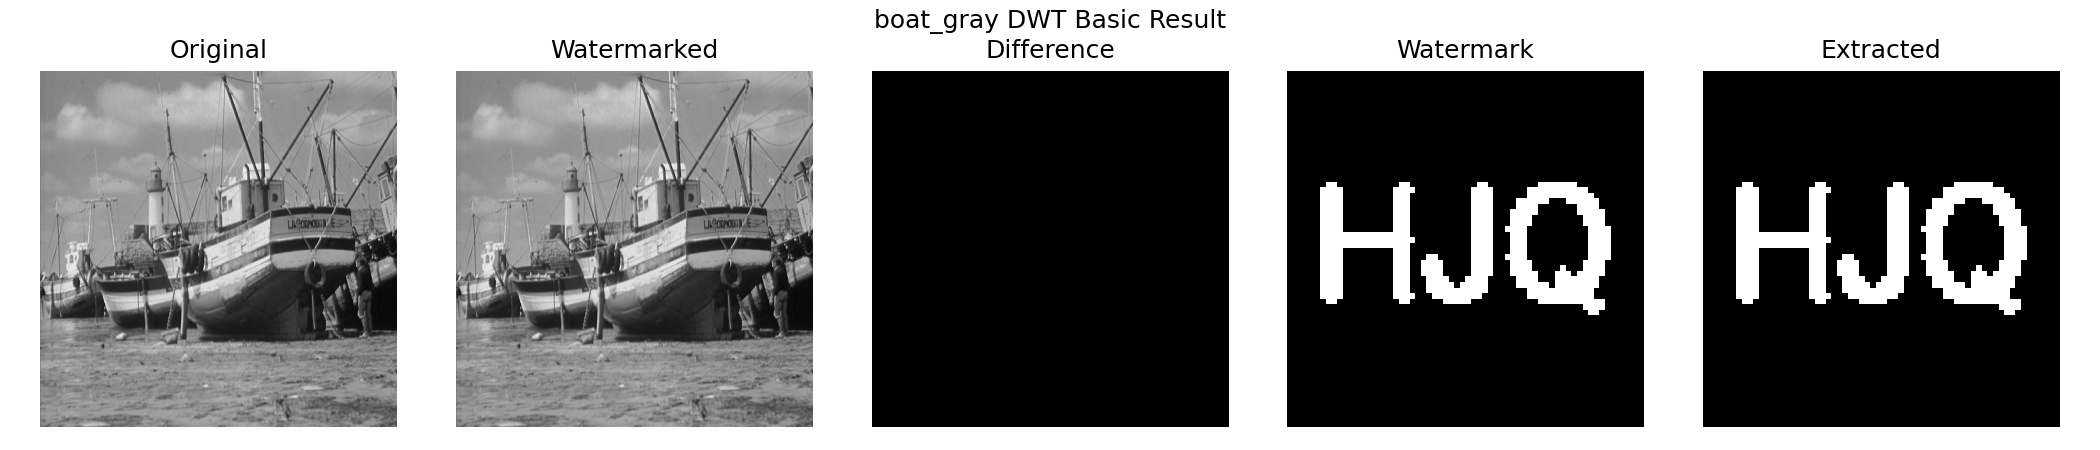
\includegraphics[width=0.95\textwidth]{outputs/multi_image/basic/boat_gray/dwt_comparison.png}
  \caption{boat\_gray 的 DWT 结果}
  \label{fig:dwt-boat}
\end{figure}

\begin{figure}[H]
  \centering
  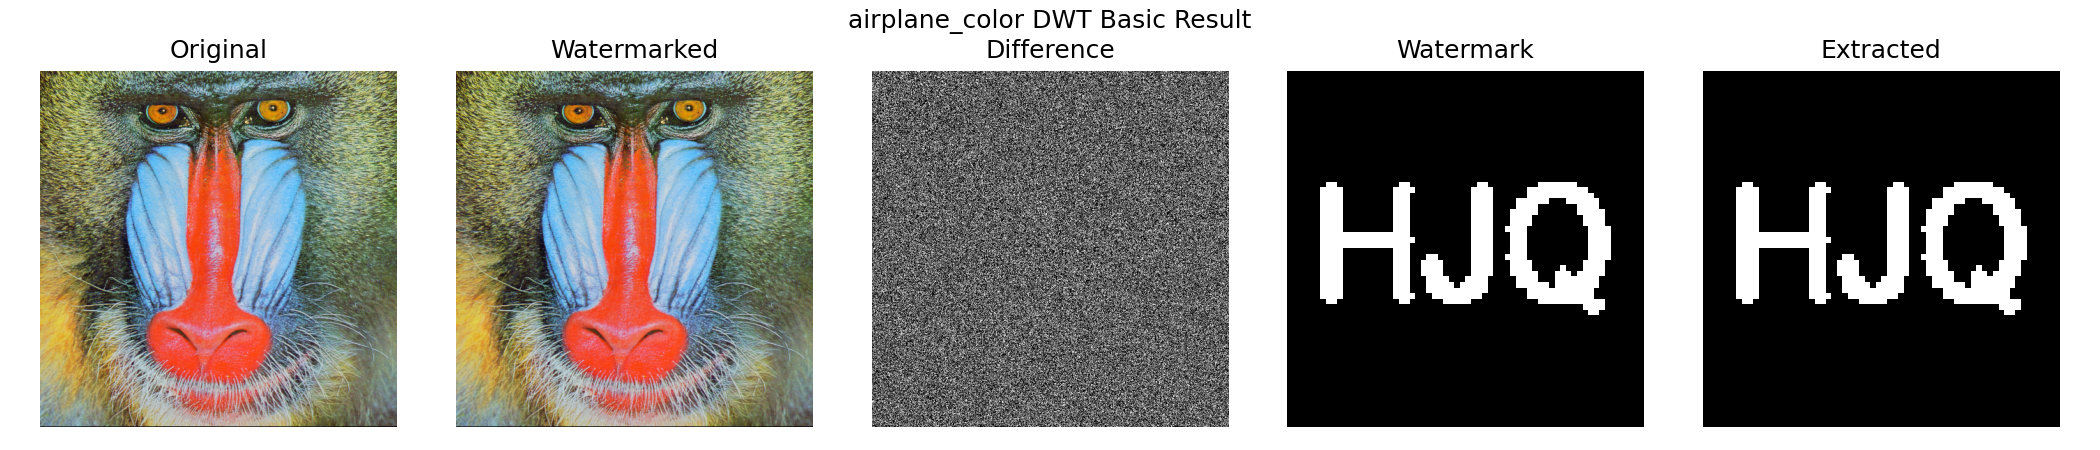
\includegraphics[width=0.95\textwidth]{outputs/multi_image/basic/airplane_color/dwt_comparison.png}
  \caption{airplane\_color 的 DWT 结果}
  \label{fig:dwt-airplane}
\end{figure}

\begin{figure}[H]
  \centering
  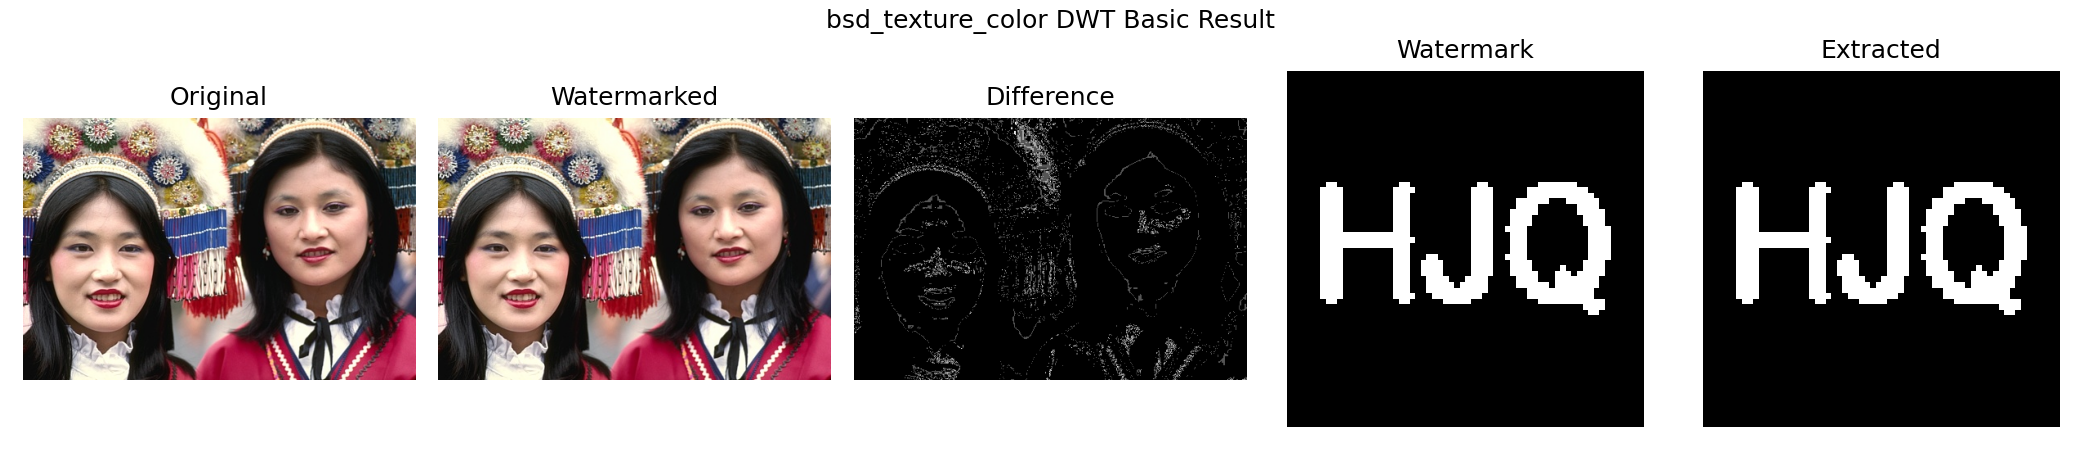
\includegraphics[width=0.95\textwidth]{outputs/multi_image/basic/bsd_texture_color/dwt_comparison.png}
  \caption{bsd\_texture\_color 的 DWT 结果}
  \label{fig:dwt-texture}
\end{figure}

\section{彩色图像 Y 通道水印接口}

\subsection{任务问题}

初版多图实验中，彩色图 bsd\_color 的输出丢失了全部颜色，原因是统一使用了 OpenCV 的灰度读取方式，彩色信息在读入时即被丢弃。对算法验证而言这无关紧要，但作为图像水印系统，“输入彩色、输出灰度”显然不可接受，因此设计了 Y 通道水印接口。

\subsection{算法设计与实现}

将 RGB 图像转换到 YCrCb 颜色空间，仅对亮度通道 Y 执行频域水印，色度通道 Cr、Cb 原样保留，处理后合成回 RGB：

\begin{lstlisting}[language=Python]
def luminance_channel(image):
    if image.ndim == 2:
        return image
    return cv2.cvtColor(image, cv2.COLOR_RGB2YCrCb)[:, :, 0]

def replace_luminance(image, luminance):
    if image.ndim == 2:
        return luminance
    ycrcb = cv2.cvtColor(image, cv2.COLOR_RGB2YCrCb)
    ycrcb[:, :, 0] = np.clip(luminance, 0, 255).astype(np.uint8)
    return cv2.cvtColor(ycrcb, cv2.COLOR_YCrCb2RGB)
\end{lstlisting}

选择 Y 通道而非对 R、G、B 三通道分别嵌入，有三方面考虑：其一，三种算法无需任何改动，它们处理的仍是二维矩阵；其二，图像结构信息集中于亮度通道，单次嵌入即可；其三，JPEG 压缩对色度通道的下采样不会波及嵌入在亮度中的水印。命令行工具相应增加 \texttt{--color-y} 选项，实验脚本对 \texttt{source\_type: color} 的图像自动启用该路径。

\subsection{运行结果与分析}

Figure~\ref{fig:y-bsd}--\ref{fig:y-landscape} 给出三张 BSD 彩色图分别经 DFT、DFT、DWT 处理后的结果，输出图像颜色完整保留，Y 通道接口达到设计目标。

\begin{figure}[H]
  \centering
  
\includegraphics[width=0.95\textwidth]{outputs/multi_image/basic/bsd_color/dft_comparison.png}
  \caption{bsd\_color 的 DFT 结果（Y 通道处理）}
  \label{fig:y-bsd}
\end{figure}

\begin{figure}[H]
  \centering
  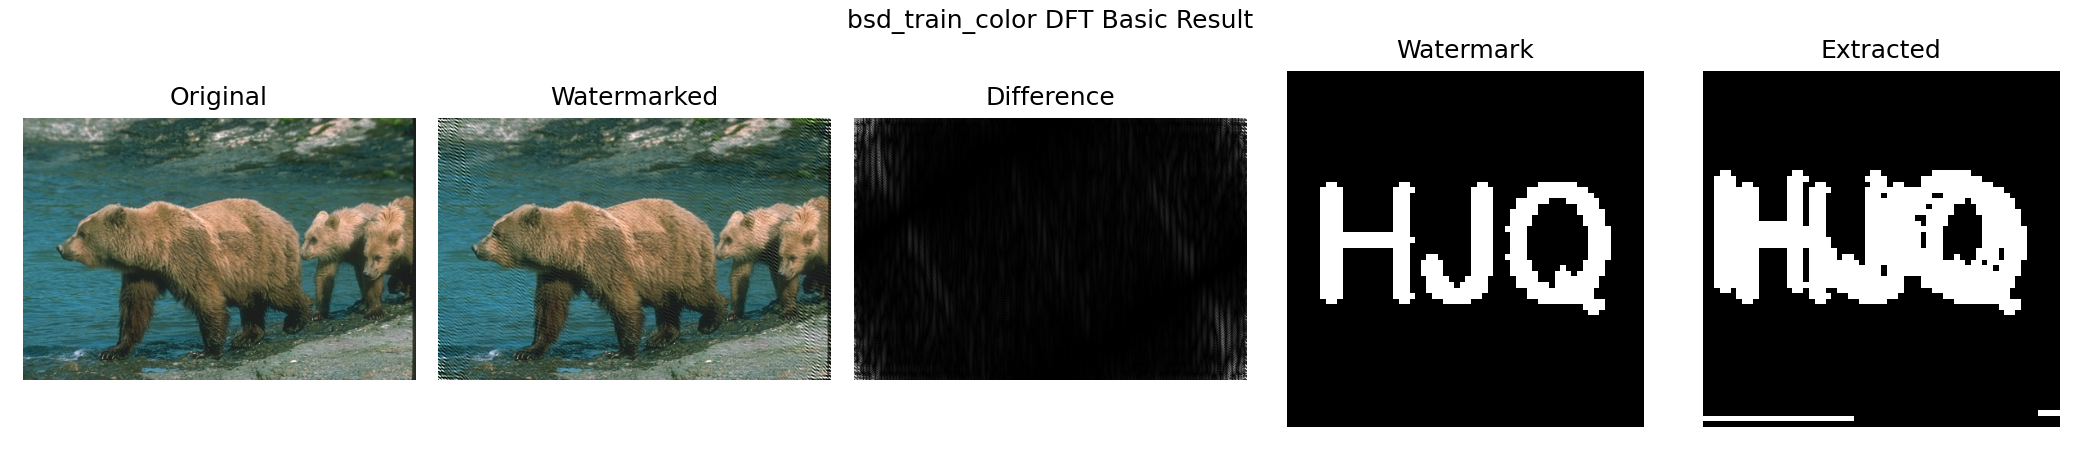
\includegraphics[width=0.95\textwidth]{outputs/multi_image/basic/bsd_train_color/dft_comparison.png}
  \caption{bsd\_train\_color 的 DFT 结果（Y 通道处理）}
  \label{fig:y-train}
\end{figure}

\begin{figure}[H]
  \centering
  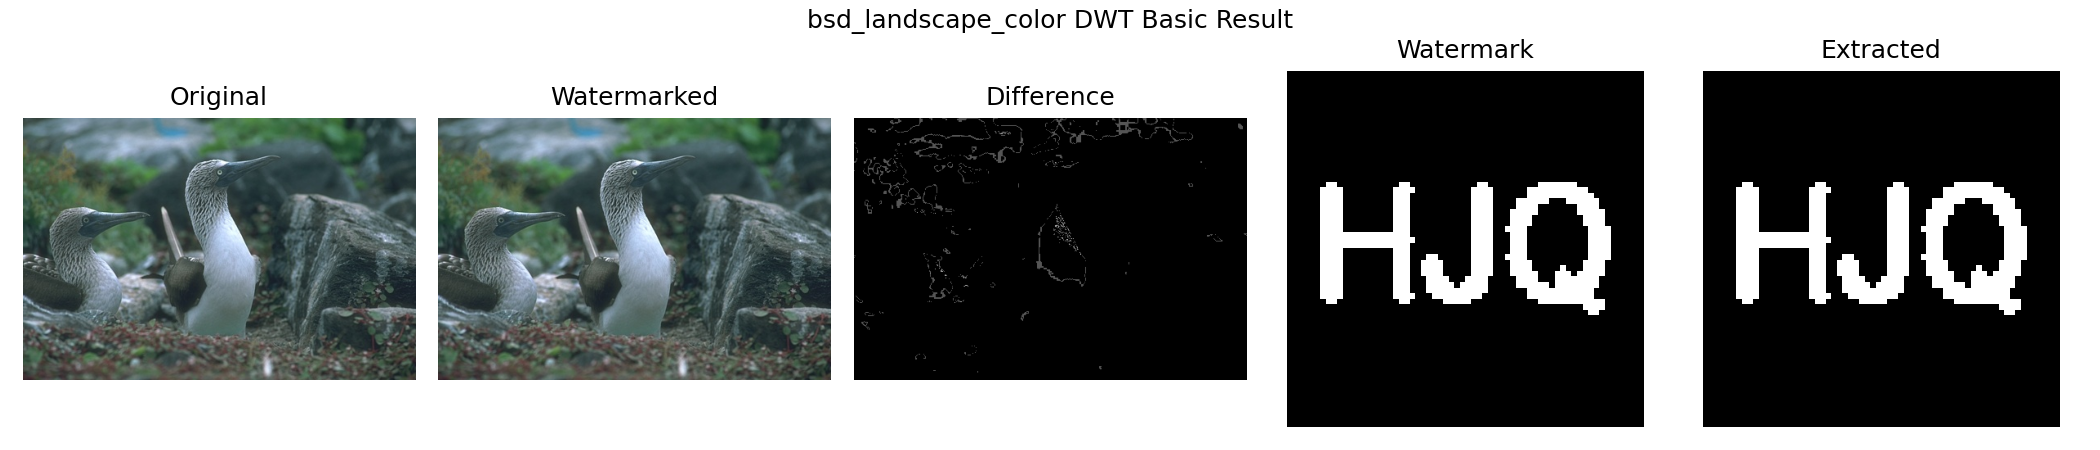
\includegraphics[width=0.95\textwidth]{outputs/multi_image/basic/bsd_landscape_color/dwt_comparison.png}
  \caption{bsd\_landscape\_color 的 DWT 结果（Y 通道处理）}
  \label{fig:y-landscape}
\end{figure}

\section{基础实验结果汇总}

\subsection{数据组织}

基础实验对 10 张图 $\times$ 3 种算法执行嵌入、提取与指标计算，每张图对应一个输出目录（含水印图、提取水印、五联对比图、频谱图与单图 CSV），汇总数据写入 \texttt{metrics\_basic\_all.csv}，共 30 行。

\subsection{平均指标}

\begin{table}[H]
  \centering
  \caption{三种算法在 10 张图上的平均指标}
  \label{tab:basic-avg}
  \begin{tabular}{lrrrrr}
    \toprule
    算法 & MSE & PSNR (dB) & SSIM & NC & BER \\
    \midrule
    DFT & 261.85 & 24.13 & 0.752 & 0.924 & 0.038 \\
    DCT & 1.61 & 47.54 & 0.996 & 0.997 & 0.001 \\
    DWT$^*$ & 0.03 & $\infty$ & 0.9999 & 1.0 & 0.0 \\
    \bottomrule
  \end{tabular}

  \vspace{4pt}
  {\footnotesize $^*$ DWT 的提取指标受 5.2 节所述同实例缓存影响，仅供参考；PSNR 为 $\infty$ 系扰动经取整后完全消失。}
\end{table}

\begin{table}[H]
  \centering
  \caption{代表性图像的单图指标}
  \label{tab:basic-single}
  \begin{tabular}{lllrrr}
    \toprule
    图像 & 尺寸 & 算法 & PSNR (dB) & SSIM & BER \\
    \midrule
    boat\_gray & $512\times512$ & DFT & 22.95 & 0.706 & 0 \\
    boat\_gray & $512\times512$ & DCT & 51.71 & 0.997 & 0 \\
    pattern\_gray & $512\times512$ & DCT & 49.45 & 0.998 & 0.0127 \\
    house\_color & $512\times512$ & DCT & 49.45 & 0.996 & 0 \\
    bsd\_color & $481\times321$ & DFT & 25.49 & 0.896 & 0.0874 \\
    bsd\_color & $481\times321$ & DCT & 44.00 & 0.997 & 0.001 \\
    \bottomrule
  \end{tabular}
\end{table}

Table~\ref{tab:basic-single} 中体现了前文分析过的两个现象：DFT 在奇数尺寸 BSD 图上的 BER 异常（3.4 节），以及 DCT 在大面积平坦的 pattern 图上的舍入损伤（4.4 节）。

\subsection{多图结果展示}

\begin{figure}[H]
  \centering
  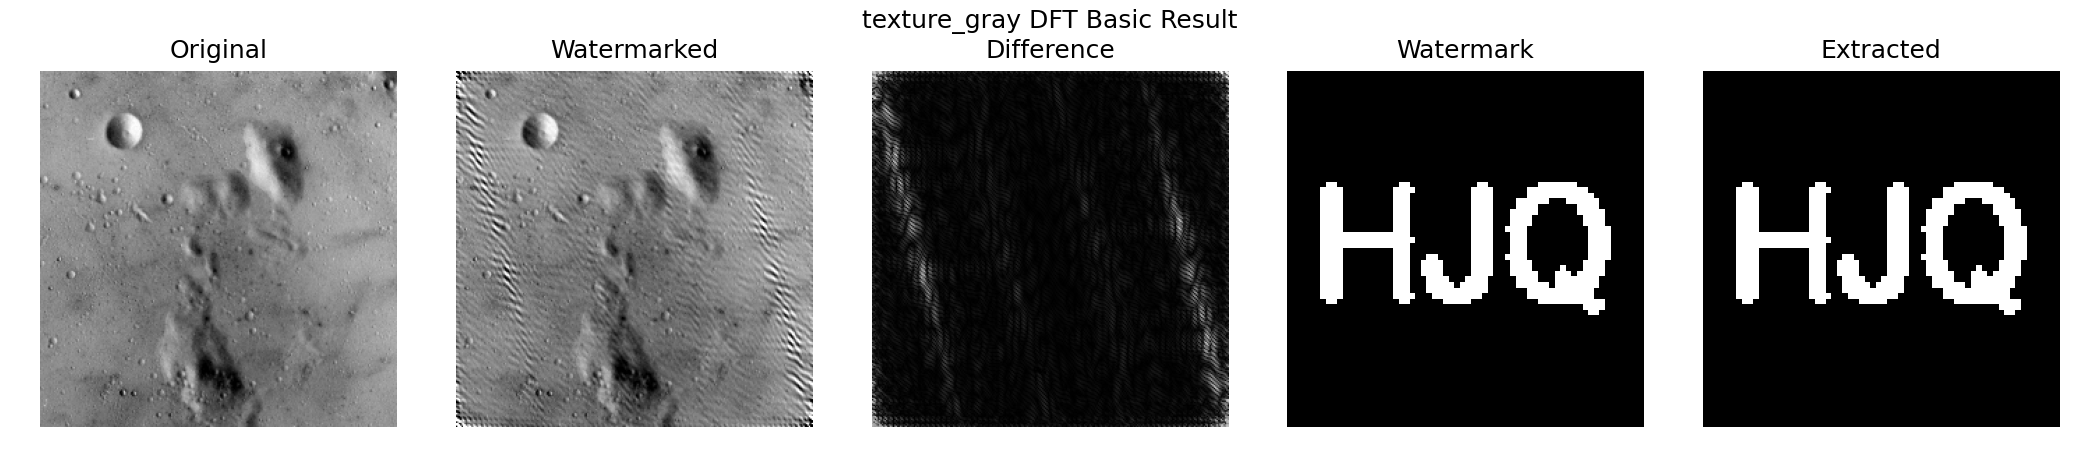
\includegraphics[width=0.95\textwidth]{outputs/multi_image/basic/texture_gray/dft_comparison.png}
  \caption{texture\_gray 的 DFT 结果}
  \label{fig:multi-texture}
\end{figure}

\begin{figure}[H]
  \centering
  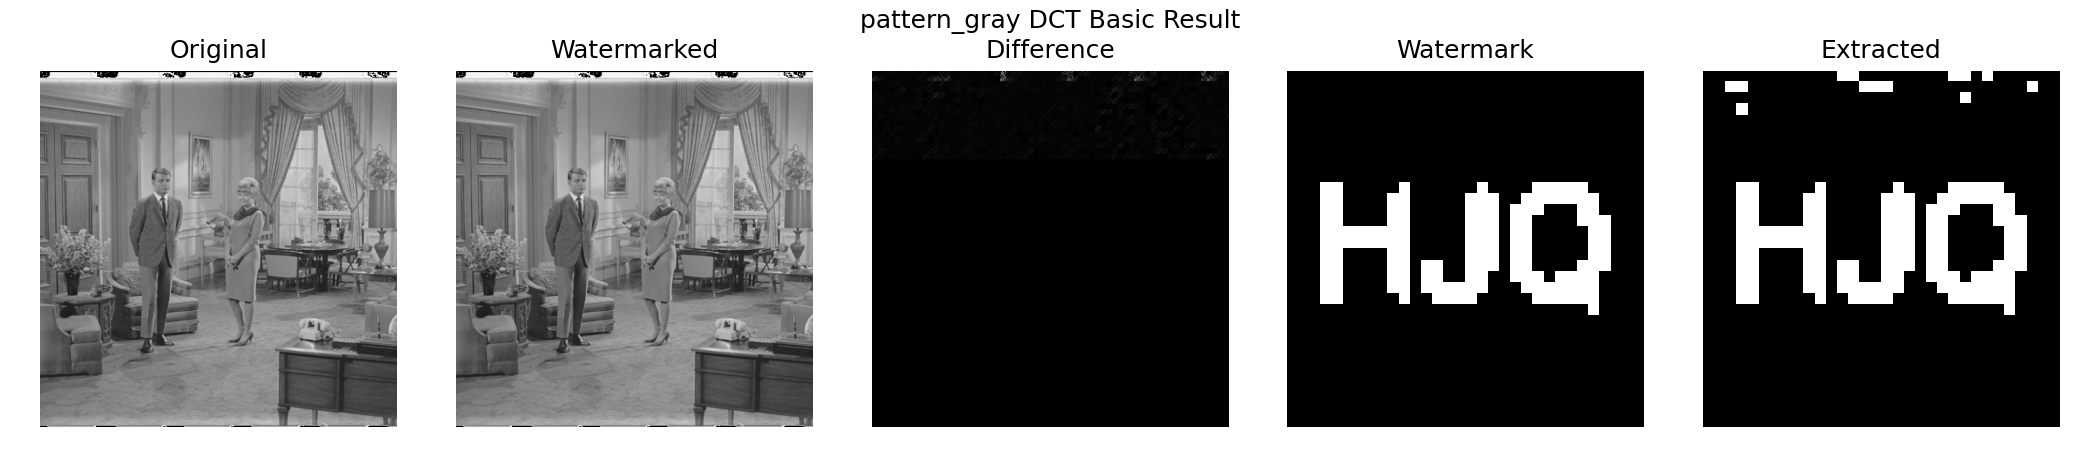
\includegraphics[width=0.95\textwidth]{outputs/multi_image/basic/pattern_gray/dct_comparison.png}
  \caption{pattern\_gray 的 DCT 结果}
  \label{fig:multi-pattern}
\end{figure}

\begin{figure}[H]
  \centering
  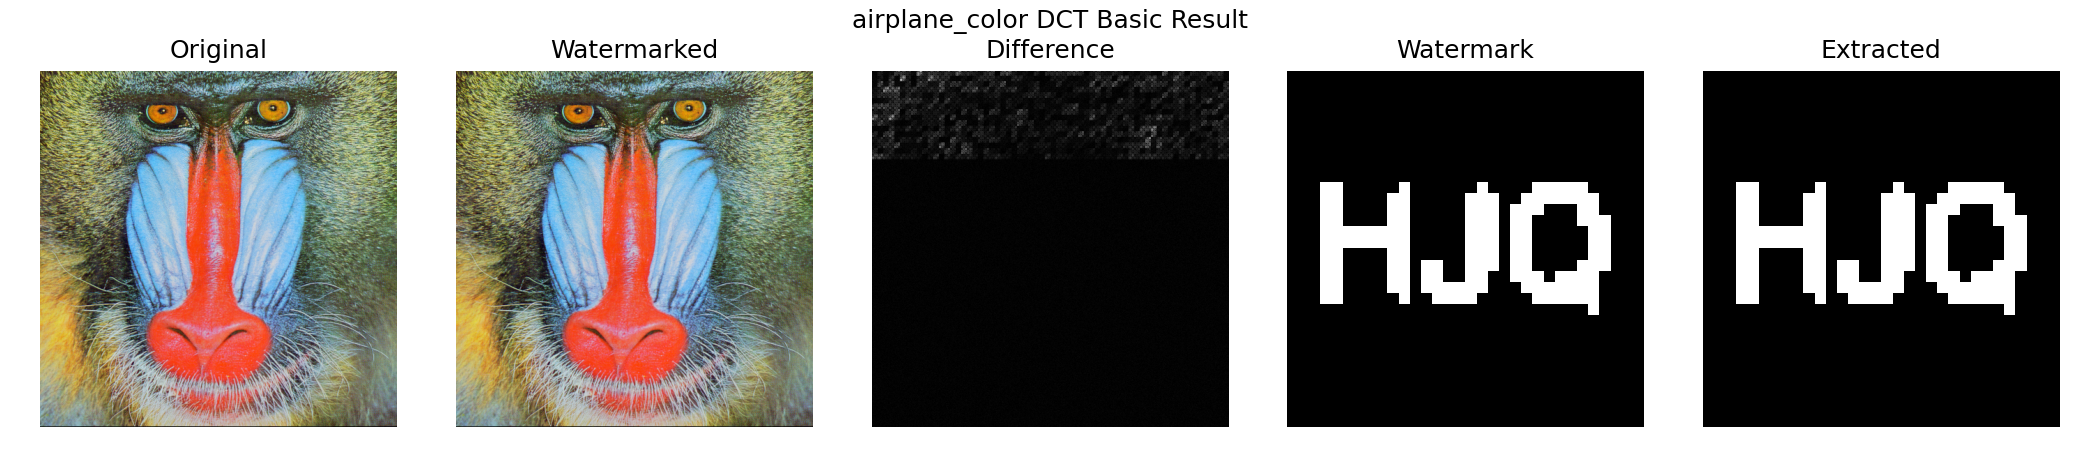
\includegraphics[width=0.95\textwidth]{outputs/multi_image/basic/airplane_color/dct_comparison.png}
  \caption{airplane\_color 的 DCT 结果}
  \label{fig:multi-airplane}
\end{figure}

\begin{figure}[H]
  \centering
  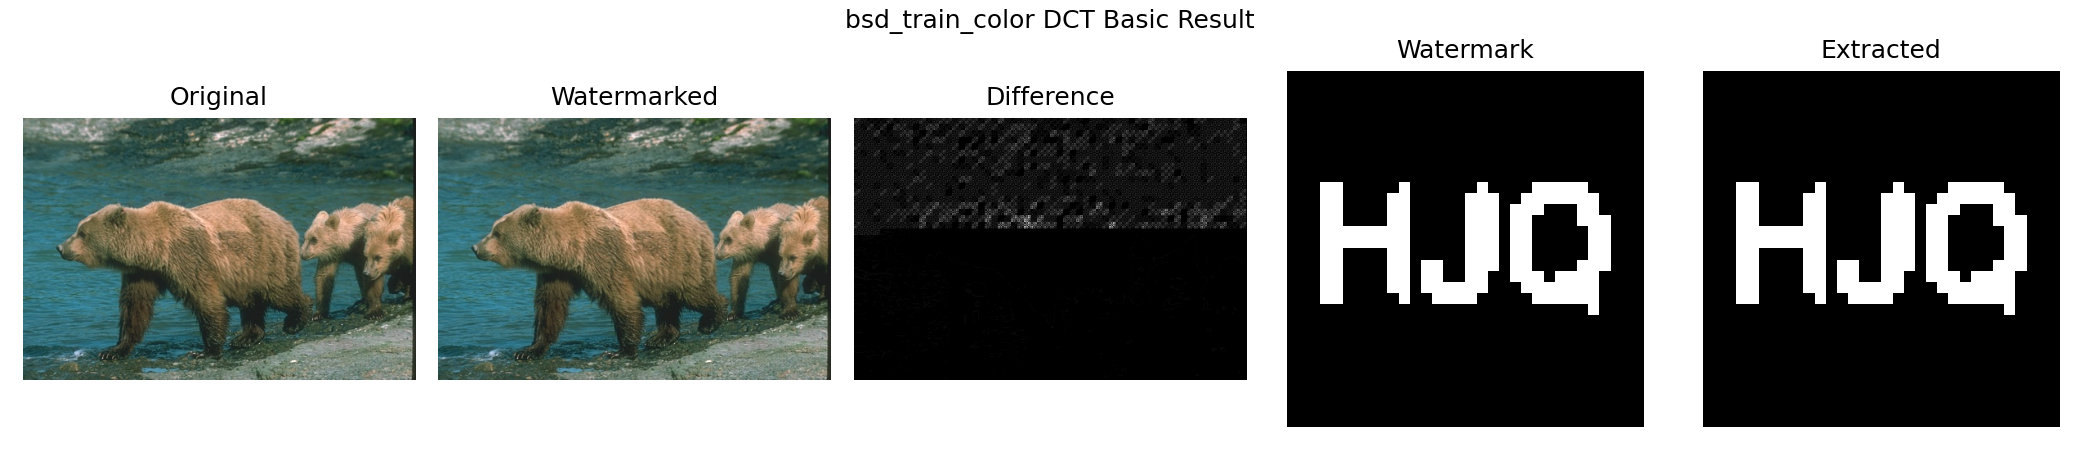
\includegraphics[width=0.95\textwidth]{outputs/multi_image/basic/bsd_train_color/dct_comparison.png}
  \caption{bsd\_train\_color 的 DCT 结果}
  \label{fig:multi-train}
\end{figure}

\begin{figure}[H]
  \centering
  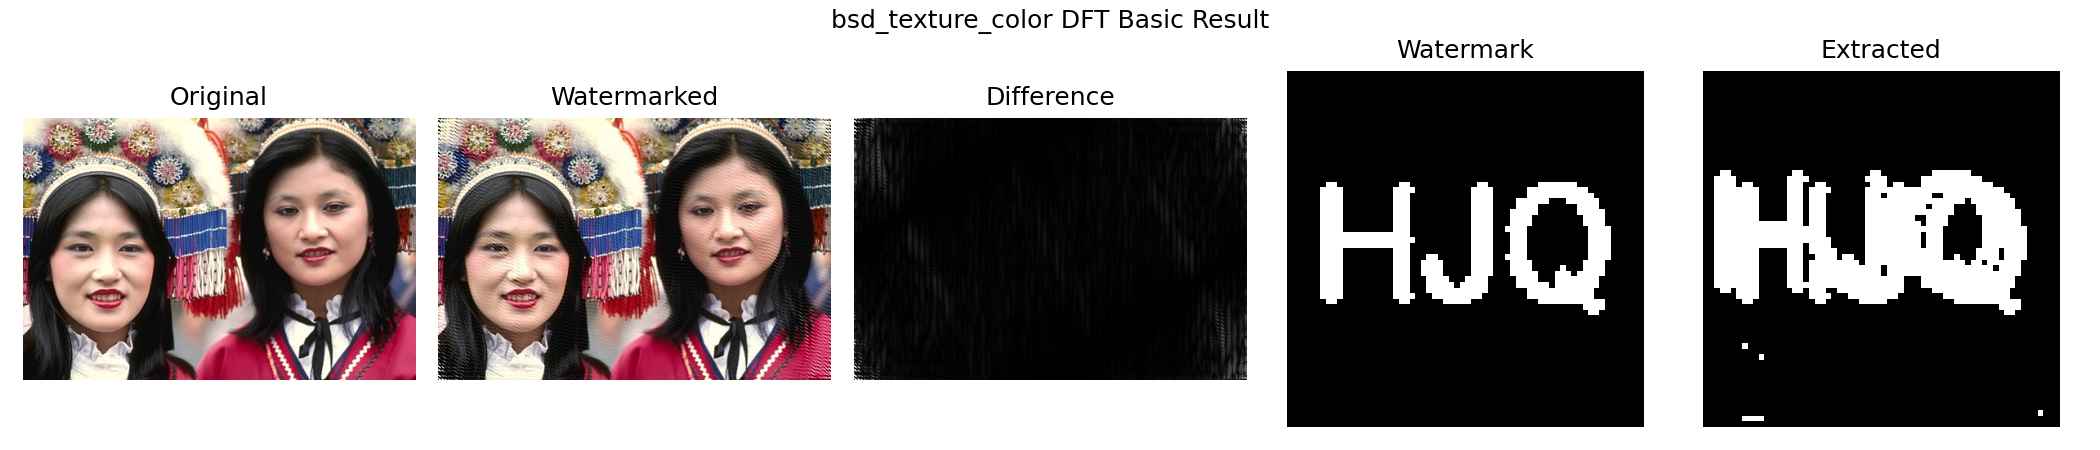
\includegraphics[width=0.95\textwidth]{outputs/multi_image/basic/bsd_texture_color/dft_comparison.png}
  \caption{bsd\_texture\_color 的 DFT 结果}
  \label{fig:multi-bsdtexture}
\end{figure}

对比不同图像可以看出纹理的掩蔽作用：texture、bsd\_texture 这类纹理繁密的图像上，同样强度的水印扰动几乎完全隐没在图像自身细节中；而 gray21、pattern 这类平坦图像上差异更易察觉，DCT 甚至因平坦块的舍入丢失比特。同一算法、同一组参数在不同内容的图像上效果可相差一个量级，这正是本实验坚持使用 10 张图而非单张图的原因。

\section{进阶任务一：嵌入强度分析}

\subsection{任务问题}

嵌入强度是水印系统中最核心的权衡参数：强度过低，水印对图像影响小但提取易出错；强度过高，提取稳定但图像失真增大。本节通过参数扫描定量分析强度对图像质量与提取准确率的影响。

\subsection{实验设计与实现}

对 DFT 与 DCT 各扫描 5 档强度（2、5、10、20、40），DWT 扫描 4 档（0.01--0.1），每档在全部 10 张图上执行嵌入与提取，共 140 行数据。实现上将强度参数覆盖入算法构造参数后走标准流程：

\begin{lstlisting}[language=Python]
for method in selected_methods:
    for value in sweep[method]:
        params = dict(config["methods"][method])
        params[_strength_key(method)] = value   # dct: delta; others: alpha
        watermarker = create_watermarker(method, **params)
        embedded = watermarker.embed(image, watermark)
        extracted = watermarker.extract(
            embedded.image, watermark.shape,
            original_image=image if method == "dft" else None)
\end{lstlisting}

\subsection{运行结果与分析}

\begin{figure}[H]
  \centering
  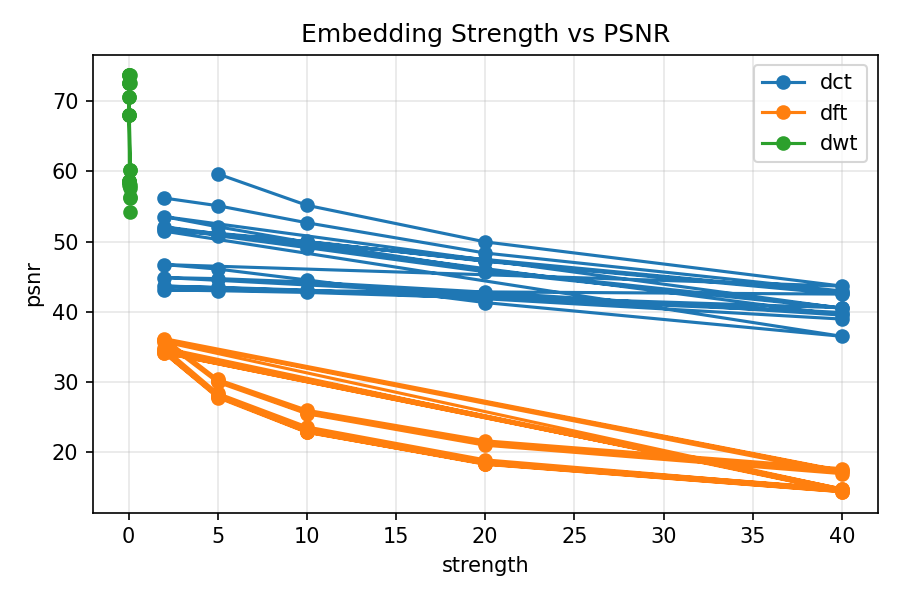
\includegraphics[width=0.78\textwidth]{outputs/multi_image/strength/strength_psnr_all.png}
  \caption{强度--PSNR 曲线（10 图平均）}
  \label{fig:strength-psnr}
\end{figure}

\begin{figure}[H]
  \centering
  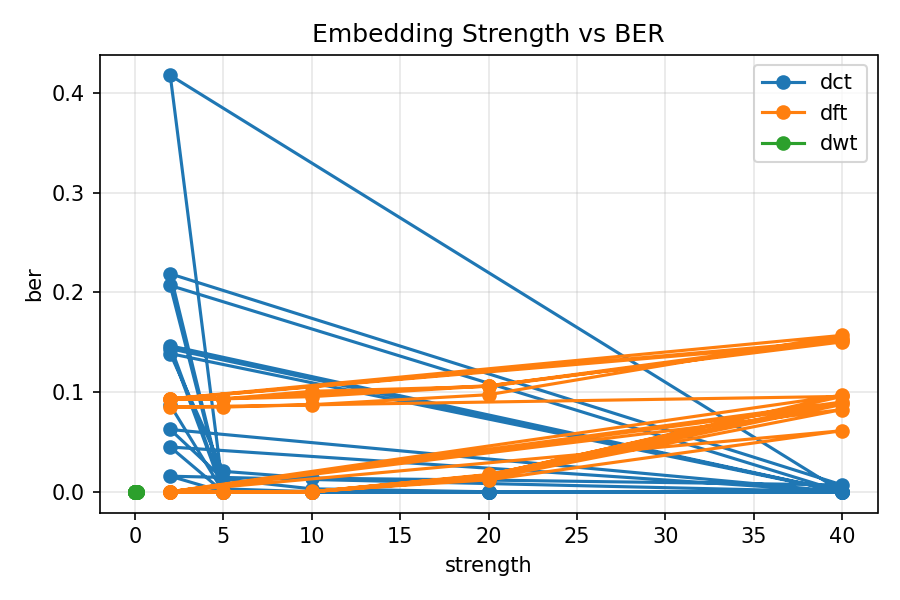
\includegraphics[width=0.78\textwidth]{outputs/multi_image/strength/strength_ber_all.png}
  \caption{强度--BER 曲线（10 图平均）}
  \label{fig:strength-ber}
\end{figure}

\begin{figure}[H]
  \centering
  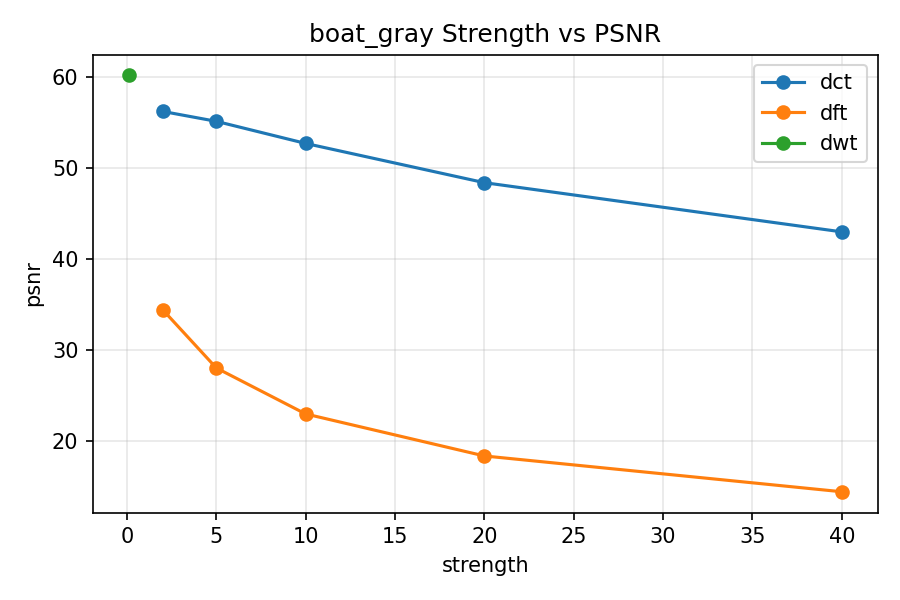
\includegraphics[width=0.72\textwidth]{outputs/multi_image/strength/boat_gray/strength_psnr.png}
  \caption{boat\_gray 的强度--PSNR 曲线}
  \label{fig:strength-boat-psnr}
\end{figure}

\begin{figure}[H]
  \centering
  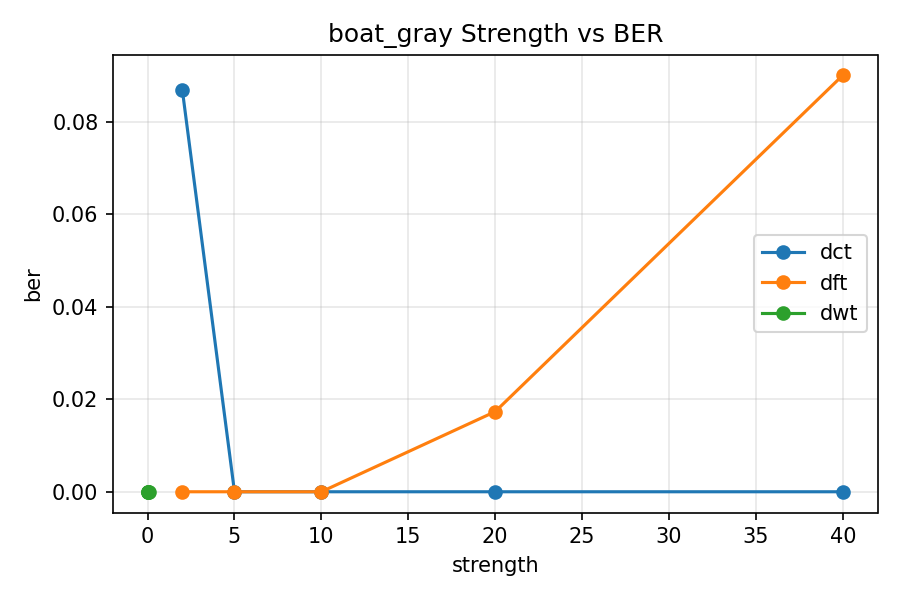
\includegraphics[width=0.72\textwidth]{outputs/multi_image/strength/boat_gray/strength_ber.png}
  \caption{boat\_gray 的强度--BER 曲线}
  \label{fig:strength-boat-ber}
\end{figure}

\begin{figure}[H]
  \centering
  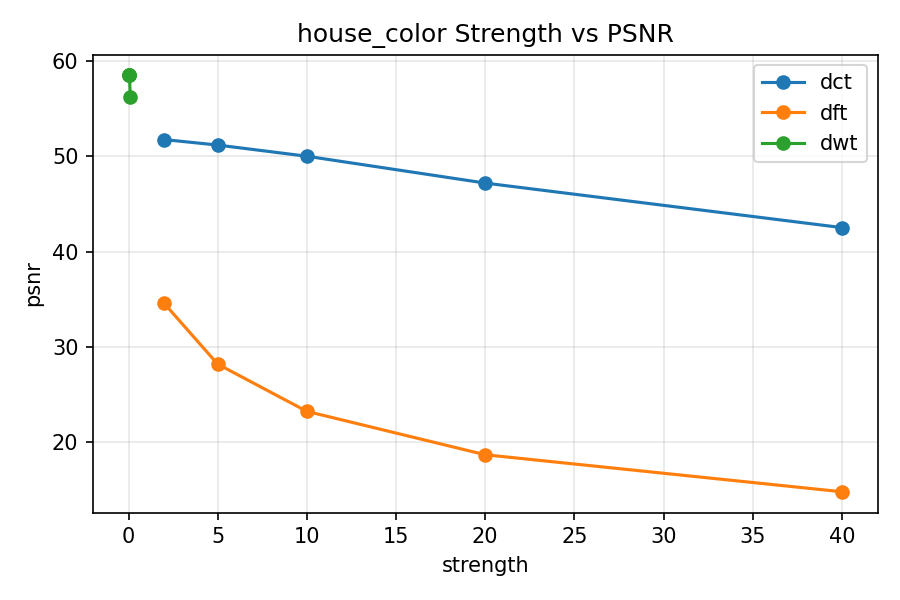
\includegraphics[width=0.72\textwidth]{outputs/multi_image/strength/house_color/strength_psnr.png}
  \caption{house\_color 的强度--PSNR 曲线}
  \label{fig:strength-house-psnr}
\end{figure}

\begin{figure}[H]
  \centering
  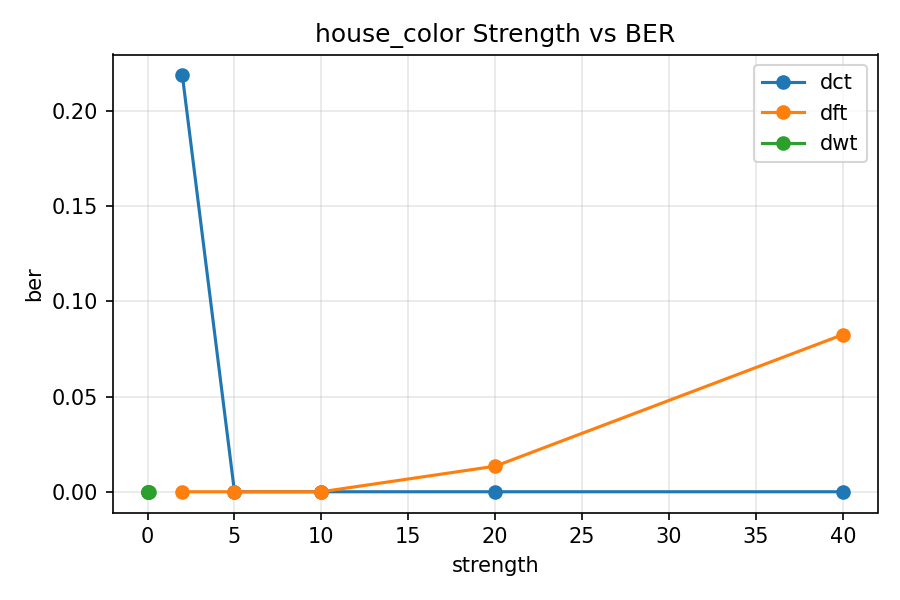
\includegraphics[width=0.72\textwidth]{outputs/multi_image/strength/house_color/strength_ber.png}
  \caption{house\_color 的强度--BER 曲线}
  \label{fig:strength-house-ber}
\end{figure}

\begin{table}[H]
  \centering
  \caption{强度实验的 10 图平均结果（DFT 参数为 $\alpha$，DCT 参数为 $\delta$）}
  \label{tab:strength}
  \begin{tabular}{rrrrr}
    \toprule
    强度 & DFT PSNR (dB) & DFT BER & DCT PSNR (dB) & DCT BER \\
    \midrule
    2 & 35.05 & 0.0365 & $\infty$ & 0.1482 \\
    5 & 28.91 & 0.0365 & 49.73 & 0.0036 \\
    10 & 24.13 & 0.0382 & 48.16 & 0.0017 \\
    20 & 19.63 & 0.0506 & 45.24 & 0.0012 \\
    40 & 15.69 & 0.1127 & 40.78 & 0.0007 \\
    \bottomrule
  \end{tabular}
\end{table}

DCT 的行为最符合理论预期：$\delta$ 从 5 增至 40，BER 由 0.36\% 降至 0.07\%，PSNR 由 49.7 dB 缓降至 40.8 dB，构成一条清晰的“鲁棒性换画质”曲线，默认值 $\delta=12$ 位于拐点附近，是合理折中。

Table~\ref{tab:strength} 中有两个反直觉的数据点值得展开分析：

\textbf{1. DCT 在 $\delta=2$ 时 PSNR 为无穷大而 BER 高达 14.8\%。}PSNR $=\infty$ 并非算法完美，恰恰相反：$\pm1$ 的系数扰动经 IDCT 与取整后完全消失，含水印图与原图逐像素相同，水印实际上没有写入图像，提取自然大面积出错。该数据点直观演示了“嵌入强度低于量化噪声地板时，嵌入等于未嵌入”。

\textbf{2. DFT 的 BER 随强度不降反升。}$\alpha=40$ 时 BER 达 11.3\%，是 $\alpha=2$ 时的三倍。原因在于动态范围：扰动过大时逆变换结果溢出 $[0,255]$，\texttt{normalize\_uint8} 为容纳溢出值对全图进行非线性重拉伸，等效于给频谱叠加了额外失真，反而破坏了部分嵌入信息。对本实现而言，“越用力越牢”在 $\alpha$ 超过 20 后即不再成立。

\section{进阶任务二：抗攻击能力测试}

\subsection{任务问题}

图像在实际传播中通常会经历压缩、缩放、加噪等处理。本节测试水印在三类攻击下的存活能力：JPEG 有损压缩（质量因子 90/70/50/30）、加性高斯噪声（$\sigma=5/10/20$）与缩放攻击（缩放至 0.5/0.75/1.5 倍后插值回原尺寸）。

\subsection{攻击模型与实现}

攻击实验先按默认强度嵌入水印，对含水印图像施加攻击，再从攻击后图像中提取：

\begin{lstlisting}[language=Python]
attacks  = [("jpeg",   q, jpeg_compress(embedded.image, q)) for q in qualities]
attacks += [("noise",  s, gaussian_noise(embedded.image, s)) for s in sigmas]
attacks += [("resize", s, resize_attack(embedded.image, s)) for s in scales]
for attack_name, level, attacked in attacks:
    extracted = watermarker.extract(
        attacked, watermark.shape,
        original_image=image if method == "dft" else None)
\end{lstlisting}

10 张图 $\times$ 3 种算法 $\times$ 10 种攻击组合，共 300 行数据。

\subsection{运行结果与分析}

\begin{figure}[H]
  \centering
  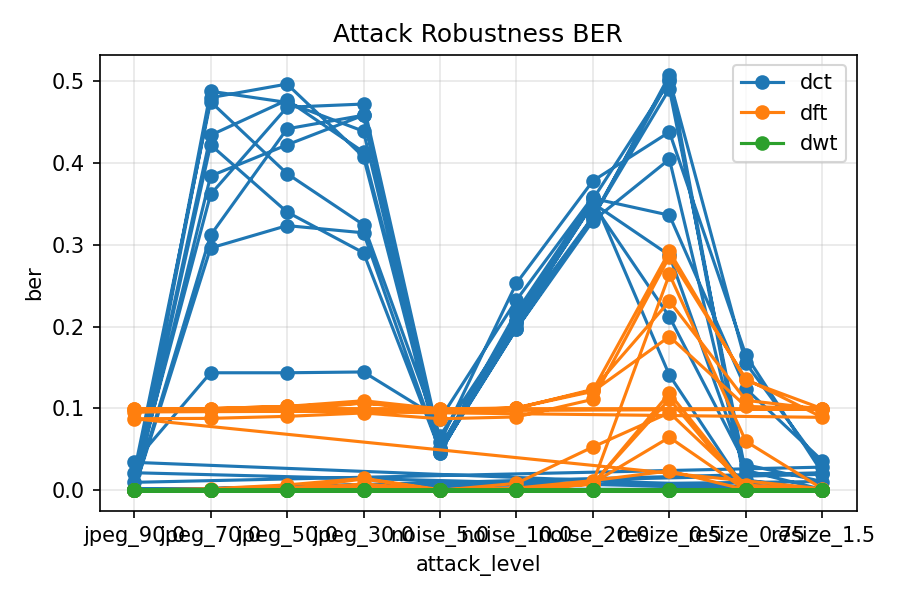
\includegraphics[width=0.82\textwidth]{outputs/multi_image/attacks/attack_ber_all.png}
  \caption{各攻击下的 BER 曲线（10 图平均；DWT 恒为 0 的曲线系 5.2 节所述缓存假象，应忽略）}
  \label{fig:attack-all}
\end{figure}

\begin{figure}[H]
  \centering
  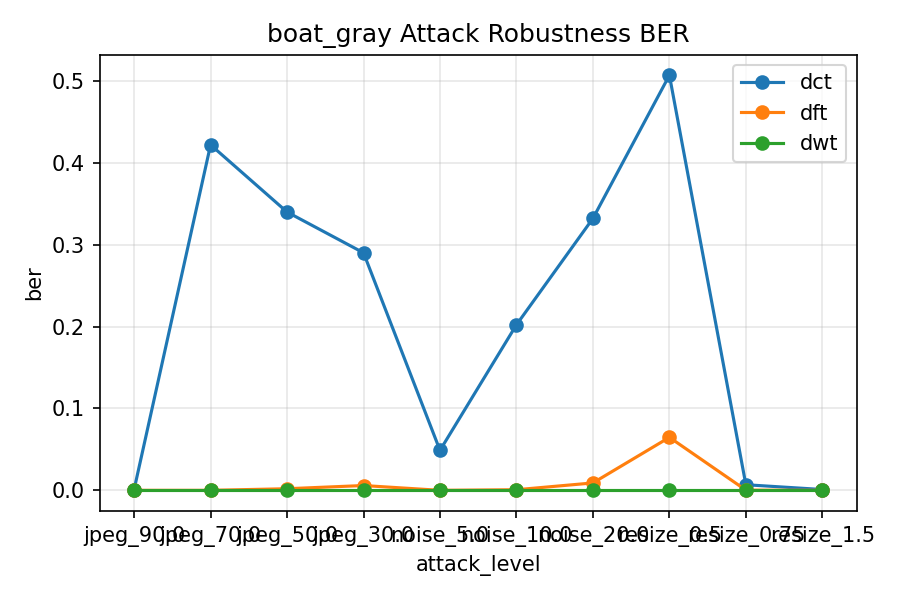
\includegraphics[width=0.75\textwidth]{outputs/multi_image/attacks/boat_gray/attack_ber.png}
  \caption{boat\_gray 的攻击--BER 曲线}
  \label{fig:attack-boat}
\end{figure}

\begin{figure}[H]
  \centering
  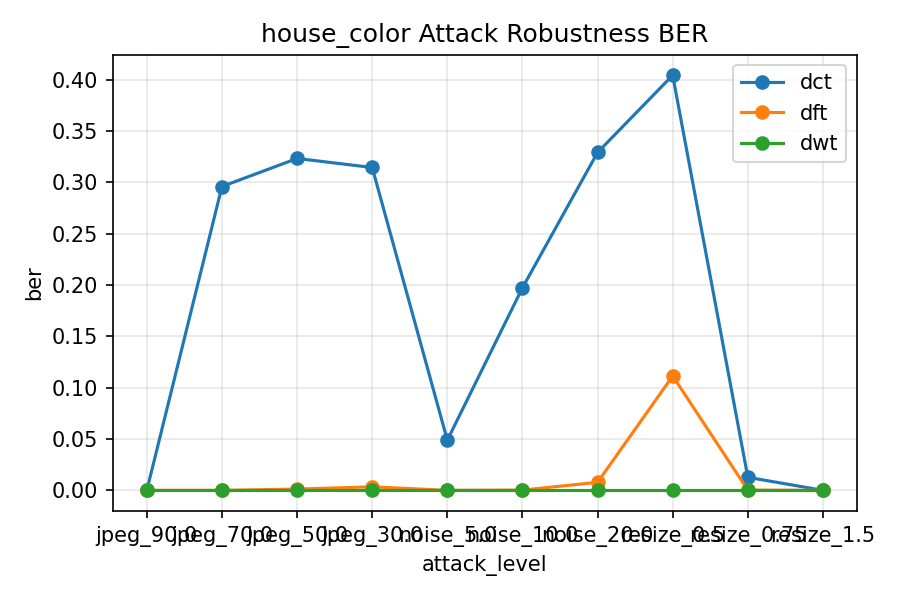
\includegraphics[width=0.75\textwidth]{outputs/multi_image/attacks/house_color/attack_ber.png}
  \caption{house\_color 的攻击--BER 曲线}
  \label{fig:attack-house}
\end{figure}

Figure~\ref{fig:attack-jpeg30}--\ref{fig:attack-noise-color} 给出部分攻击后的图像示例，可直观感受各攻击的破坏强度。

\begin{figure}[H]
  \centering
  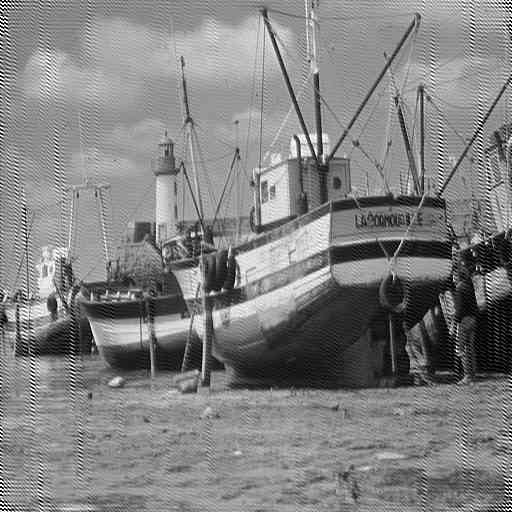
\includegraphics[width=0.5\textwidth]{outputs/multi_image/attacks/boat_gray/dft_jpeg_30_attacked.png}
  \caption{JPEG 质量 30 压缩后的 boat\_gray（DFT 含水印图）}
  \label{fig:attack-jpeg30}
\end{figure}

\begin{figure}[H]
  \centering
  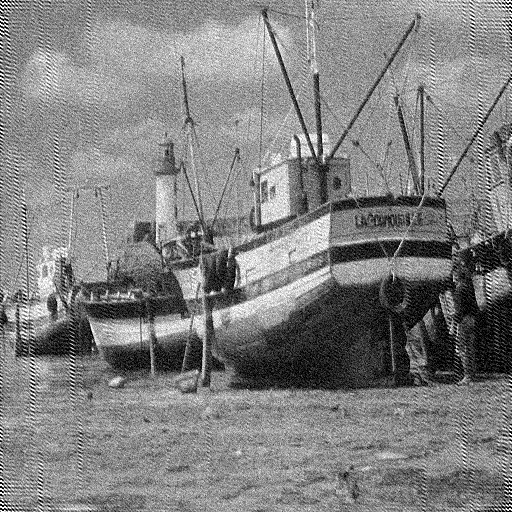
\includegraphics[width=0.5\textwidth]{outputs/multi_image/attacks/boat_gray/dft_noise_20_attacked.png}
  \caption{高斯噪声 $\sigma=20$ 后的 boat\_gray（DFT 含水印图）}
  \label{fig:attack-noise20}
\end{figure}

\begin{figure}[H]
  \centering
  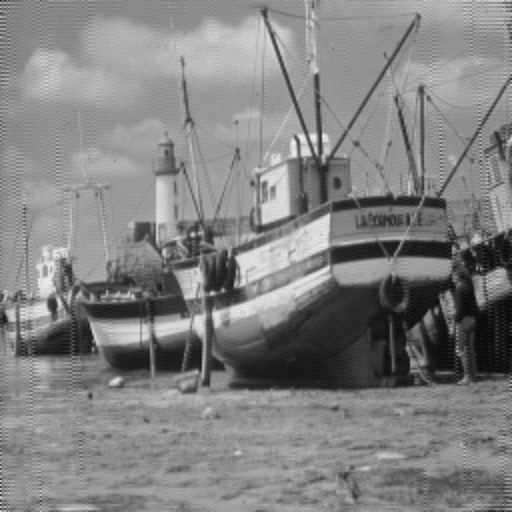
\includegraphics[width=0.5\textwidth]{outputs/multi_image/attacks/boat_gray/dft_resize_0.5_attacked.png}
  \caption{缩放 0.5 倍再恢复后的 boat\_gray（DFT 含水印图）}
  \label{fig:attack-resize05}
\end{figure}

\begin{figure}[H]
  \centering
  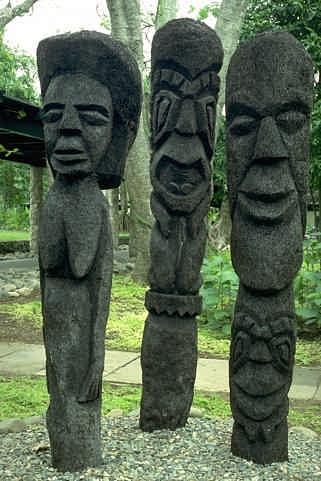
\includegraphics[width=0.5\textwidth]{outputs/multi_image/attacks/bsd_color/dct_jpeg_30_attacked.png}
  \caption{JPEG 质量 30 压缩后的 bsd\_color（DCT 含水印图）}
  \label{fig:attack-jpeg-color}
\end{figure}

\begin{figure}[H]
  \centering
  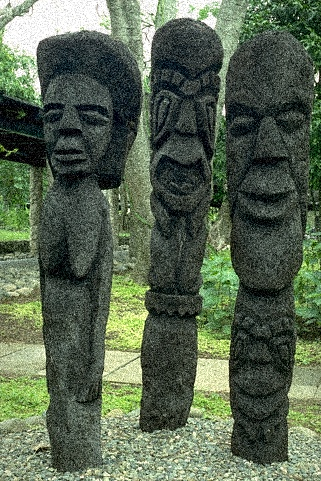
\includegraphics[width=0.5\textwidth]{outputs/multi_image/attacks/bsd_color/dct_noise_20_attacked.png}
  \caption{高斯噪声 $\sigma=20$ 后的 bsd\_color（DCT 含水印图）}
  \label{fig:attack-noise-color}
\end{figure}

\begin{table}[H]
  \centering
  \caption{各攻击档位下的 10 图平均 BER 与 NC（DWT 数据因缓存机制不具参考性，不列入）}
  \label{tab:attack}
  \begin{tabular}{llrrrr}
    \toprule
    攻击 & 档位 & DCT BER & DCT NC & DFT BER & DFT NC \\
    \midrule
    JPEG & 90 & 0.007 & 0.986 & 0.038 & 0.924 \\
    JPEG & 70 & 0.379 & 0.241 & 0.039 & 0.922 \\
    JPEG & 50 & 0.397 & 0.206 & 0.041 & 0.919 \\
    JPEG & 30 & 0.372 & 0.256 & 0.047 & 0.906 \\
    噪声 & $\sigma=5$ & 0.055 & 0.890 & 0.038 & 0.923 \\
    噪声 & $\sigma=10$ & 0.213 & 0.573 & 0.040 & 0.919 \\
    噪声 & $\sigma=20$ & 0.348 & 0.305 & 0.058 & 0.885 \\
    缩放 & 0.5 & 0.382 & 0.237 & 0.167 & 0.666 \\
    缩放 & 0.75 & 0.054 & 0.892 & 0.055 & 0.889 \\
    缩放 & 1.5 & 0.012 & 0.976 & 0.039 & 0.922 \\
    \bottomrule
  \end{tabular}
\end{table}

\textbf{1. DCT 对 JPEG 的表现是一道断崖。}质量 90 时 BER 仅 0.7\%，质量 70 时即崩至 37.9\%。其机制可以从量化角度解释：JPEG 的量化步长随质量因子降低而增大，质量 90 时中频系数的量化步长仍小于间距 $\delta=12$，$C(3,4)$ 与 $C(4,3)$ 的顺序得以保持；至质量 70，步长已超过 $\delta$，两系数常被量化到同一格子，顺序关系近乎随机。注意质量 50 的 BER（0.397）反而高于质量 30（0.372）——这并非规律，而是两档均已落入“提取失败”区间后的随机涨落，BER 在 0.4 附近浮动（未达 0.5 是因纯平块碰巧保持顺序），具体数值不再具有可比性。

\textbf{2. 噪声与缩放攻击下 DCT 平滑退化且存在明显不对称性。}噪声 $\sigma=5$ 时 BER 5.5\% 尚可辨认，$\sigma=10$ 起迅速恶化。缩放攻击中，放大 1.5 倍再缩回几乎无损（BER 1.2\%），因为插值是平滑操作，不破坏中频系数的相对大小；缩小 0.5 倍则先丢弃了一半以上的高频信息，块结构也彻底错位，BER 崩至 38.2\%。

\textbf{3. DFT 的鲁棒性需与其基线对照评估。}表中 DFT 各 JPEG 档位 BER 稳定在 4\%--5\%，但无攻击时其平均 BER 已有 3.8\%（全部来自奇数尺寸 BSD 图，见 3.4 节），即 JPEG 压缩给 DFT 实际增加的错误不足 1 个百分点。写入中频环带、且有原图辅助对消的水印确实难以被压缩和噪声动摇；其唯一明显失分项是 0.5 倍缩放（BER 16.7\%），下采样将部分嵌入频点直接混叠掉了。

综合来看：若验证端可获得原图，DFT 非盲方案在多数攻击下更稳定；若必须盲提取，DCT 方案在轻度处理（JPEG 质量 $\ge90$、$\sigma\le5$ 噪声、0.75 倍以内缩放）下可用，面对更强攻击则需按第 8 节结论提高 $\delta$，或引入纠错编码与多数投票机制。

\section{综合讨论}

\subsection{三种算法的对比分析}

\begin{table}[H]
  \centering
  \caption{三种算法综合对比}
  \label{tab:compare}
  \begin{tabular}{lp{2cm}p{4cm}p{4cm}p{2.6cm}}
    \toprule
    算法 & 是否盲提取 & 优点 & 缺点 & 定位 \\
    \midrule
    DFT & 否 & 频域思想直观，抗压缩与噪声能力强 & 提取需原图；默认强度下失真较明显 & 基础任务与非盲基线 \\
    DCT & 是 & 不需原图；画质近乎无损；机制与 JPEG 同源，解释性强 & 对重压缩、强噪声、下采样敏感 & 挑战任务核心算法 \\
    DWT & 展示性 & 多分辨率分析；扰动极小 & 跨实例盲提取方案粗糙 & 挑战部分扩展 \\
    \bottomrule
  \end{tabular}
\end{table}

三种算法放在一起比较，结论可以概括为：没有全能的水印，只有与场景匹配的水印。DFT 将水印摊在全局频谱的中频环带上，抗压缩抗噪声，但需要原图且失真最明显；DCT 用局部块的系数顺序编码，画质与部署灵活性最好，但顺序关系在重压缩与下采样面前脆弱；DWT 展示了多分辨率域的可行性。

\subsection{参数选择建议}

DCT 的 $\delta$ 是最重要的可调参数：过小导致嵌入被取整噪声吞没（$\delta=2$ 时 BER 14.8\%），过大降低 PSNR，默认 $\delta=12$ 在本实验中兼顾画质与准确率；若预期图像将经历质量低于 90 的 JPEG 重压缩，应将 $\delta$ 提高到 20 以上并配合纠错编码。DFT 的 $\alpha$ 存在有效上限，超过 20 后归一化重拉伸反而使 BER 上升，不宜盲目增大。

\subsection{局限与改进方向}

本项目当前存在的局限包括：DFT 在奇数尺寸图像上的镜像错位已定位但未修复；DCT 对低方差平坦块的舍入丢比特未做规避；DWT 缺乏可靠的跨实例盲提取；所有方案均无纠错编码；面对裁剪、旋转等几何攻击缺少同步机制。改进优先级上，为 DCT 增加纠错码与低方差块跳过的改动小、收益直接；更长期的方向包括 DWT--DCT--SVD 混合水印与基于特征点的几何同步。

\subsection{总结与展望}

本实验围绕图像频域水印完成了覆盖基础、进阶、挑战三个层次的完整系统：基础任务以 DFT 走通频域嵌入、逆变换、非盲提取全流程；进阶任务以 140 组强度数据与 300 组攻击数据刻画了画质--鲁棒性权衡；挑战任务实现了不需原图的 DCT 盲水印，并扩展了 DWT 方法与彩色 Y 通道接口。全部实验由配置驱动、脚本一键复现，26 个自动化测试保障主要功能正确性。

实验中的若干反常数据点（奇数尺寸的 DFT 错位、$\delta=2$ 时 PSNR 为无穷大、$\alpha$ 过大时 BER 回升、JPEG 质量 90 与 70 之间的断崖）经逐一分析均得到了机制层面的解释，这些分析加深了我们对采样、量化与频域变换之间相互作用的理解。未来工作可沿纠错编码、自适应嵌入与几何同步方向继续推进。

\section{成员分工}

本项目由侯治民、乔义杰、金灏、王师睿四人完成，分工按照“核心开发者承担实现与集成，其他组员分别负责实验、测试与文档”的方式组织，详见 Table~\ref{tab:work}。

\begin{longtable}{p{7.2cm}cccc}
  \caption{分工安排详表}\label{tab:work}\\
  \toprule
  任务 & 侯治民 & 乔义杰 & 金灏 & 王师睿 \\
  \midrule
  \endfirsthead
  \caption[]{分工安排详表（续）}\\
  \toprule
  任务 & 侯治民 & 乔义杰 & 金灏 & 王师睿 \\
  \midrule
  \endhead
  \bottomrule
  \endfoot
  \multicolumn{5}{l}{\textbf{Coding 部分}} \\
  架构设计与算法基类 & 1.5 & & & \\
  DFT 算法实现 & 2 & & & \\
  DCT 盲水印实现 & 2 & & & \\
  DWT 扩展实现 & 1 & & & \\
  彩色 Y 通道接口 & 1 & & & \\
  攻击与指标模块 & 1.5 & & 0.5 & \\
  CLI 与配置系统 & 1.5 & & & \\
  自动化测试 & 0.5 & & & 1 \\
  \multicolumn{5}{l}{\textbf{实验部分}} \\
  数据集筛选与整理 & & 2 & & \\
  基础实验运行与结果检查 & & 2.5 & & \\
  对比图与频谱图核对 & & 1.5 & & \\
  嵌入强度实验 & & & 2.5 & \\
  抗攻击实验 & & & 2.5 & \\
  CSV 统计与曲线核对 & & 0.5 & 1.5 & \\
  \multicolumn{5}{l}{\textbf{Report 部分}} \\
  引言与系统设计章节 & 1 & & & \\
  基础任务章节 & & 1 & & \\
  进阶任务章节 & & & 0.5 & \\
  挑战任务章节 & 1.5 & & & \\
  统稿与 \LaTeX{} 排版 & 2 & & & \\
  文字校对 & & & & 1.5 \\
  \multicolumn{5}{l}{\textbf{项目开展及最终提交}} \\
  README 与使用手册 & & & & 2 \\
  requirements 与运行说明 & & & & 1 \\
  GitHub 仓库维护 & 1.5 & & & \\
  答辩 PPT & & 0.5 & & 0.5 \\
  \midrule
  合计工作量 & 17 & 8 & 7.5 & 6 \\
  \textbf{工作量占比} & \textbf{44.2\%} & \textbf{20.8\%} & \textbf{19.5\%} & \textbf{15.6\%} \\
\end{longtable}

\section{大模型使用说明}

在项目开发过程中，我们在多个环节利用了大模型（Claude Code）进行辅助，具体应用场景如下：

\begin{enumerate}
  \item \textbf{工程框架搭建}：借助大模型获取项目模块划分、算法注册表模式与配置系统的框架建议，并在此基础上针对性调整，以适配本项目的可切换算法需求；
  \item \textbf{实验脚本编写辅助}：批量实验脚本与 CSV、曲线输出的初始版本由大模型辅助生成，随后根据实验需求调整参数与输出格式，全部脚本经组员实际运行验证；
  \item \textbf{调试辅助}：在 DFT 嵌入强度随图像尺寸缩放、BER 阈值兼容性等问题的定位过程中，借助大模型分析异常现象并提出修改建议，最终修改均经自动化测试确认；
  \item \textbf{文档与排版}：README、使用手册与本报告的 \LaTeX{} 排版由大模型辅助完成，全部内容由组员审核校对，实验数据均来自实际运行结果。
\end{enumerate}

\begin{thebibliography}{9}

\bibitem{cox} I. J. Cox, M. L. Miller, J. A. Bloom, J. Fridrich, and T. Kalker. \textit{Digital Watermarking and Steganography}. 2nd ed., Morgan Kaufmann, 2008.

\bibitem{oppenheim} A. V. Oppenheim, A. S. Willsky, and S. H. Nawab. \textit{Signals and Systems}. 2nd ed., Prentice Hall, 1996.

\bibitem{sipi} USC-SIPI Image Database. Available: \url{https://sipi.usc.edu/database/}

\bibitem{bsd} D. Martin, C. Fowlkes, D. Tal, and J. Malik. A Database of Human Segmented Natural Images and its Application to Evaluating Segmentation Algorithms. In \textit{Proc. ICCV}, 2001.

\bibitem{pywt} G. R. Lee, R. Gommers, F. Waselewski, K. Wohlfahrt, and A. O'Leary. PyWavelets: A Python package for wavelet analysis. \textit{Journal of Open Source Software}, 4(36):1237, 2019.

\bibitem{opencv} OpenCV Documentation. Available: \url{https://docs.opencv.org/}

\end{thebibliography}

\end{document}
